\chapter{条件期望与条件分布}
\label{chap:conditional-expectation}

设想一台传感器只报告目标落在哪个区段，而不报告精确位置；或者一个分类器只看到图像的几项特征，看不到生成图像的全部细节。
我们仍想根据已有的观测，给出某个数值量的最好平均估计，甚至给出它在当前观测下的整个概率分布。
当观测只有有限个取值时，做法很朴素：把样本点按观测值分组，组内求平均，组内的频率归一化后就是条件分布。
可是观测一旦取连续值，每个具体取值$\{Y=y\}$的概率都是零，“组内总量除以组的概率”变成了$0/0$。
那么给定$Y=y$时的平均值究竟指什么？它在多大程度上被唯一确定？能否用同一个对象同时给出所有事件的条件概率？

本章用两项要求回答第一个问题：条件平均只能使用已有的信息，并且在每个可以观察的事件上保持原变量的积分总量。
这两项要求不涉及任何除法，因此对零概率的观测值同样有意义；第~\ref{chap:densities-change-of-measure}章的Radon--Nikodym定理保证满足它们的随机变量存在，并且几乎处处唯一。
随后我们从这两项要求推出条件期望的运算规则、嵌套信息下的塔式法则、条件均方误差的分解，以及固定信息下交换条件期望与极限的条件。

第二个问题需要换一个对象。
条件期望逐个处理可积变量，每个事件的条件概率各自只在几乎处处意义下确定；要让它们在每个观测值处拼成一个概率分布，需要“输入一个状态、输出一个概率分布”的概率核。
因此我们先独立建立概率核及其积分、联合分布与复合，再用它定义条件分布，讨论存在所需的空间条件、不同版本之间的关系，以及条件密度与Bayes公式。
最后，条件分布让我们能够准确表达“给定已有信息后，另一项观测是否还会改变分布”，这就是条件独立。

\section{信息与条件平均}
\label{sec:cond-information}

本节从只能看到分组的情形出发，确定条件平均应当满足什么要求，再用子$\sigma$代数描述“可用信息”。
这里只建立问题；生成$\sigma$代数等记号沿用第~\ref{chap:probability-models}章。

\subsection{分组观察与条件平均}

\paragraph{只看到分组时的平均}
设$(\Omega,\mathcal F,\mathbb P)$是有限概率空间，$X$是其上的随机变量。
假设观察者只能确定样本点落在划分$A_1,\ldots,A_m$中的哪一块，看不到块内的细节。
对$\mathbb P(A_i)>0$的块，最自然的估计是组内平均
\begin{equation}
  \frac{\mathbb E[X\mathbb I_{A_i}]}{\mathbb P(A_i)}=\frac{1}{\mathbb P(A_i)}\sum_{\omega\in A_i}X(\omega)\mathbb P(\{\omega\}).
  \label{eq:cond-group-average}
\end{equation}
把每一块上的组内平均放回该块，就得到一个在各块上取常值的随机变量$Z$：样本点落在$A_i$时，$Z$取式~\eqref{eq:cond-group-average}的值。

\begin{example}[四点空间上的分组平均]
\label{ex:cond-four-points}
取$\Omega=\{0,2,4,6\}$，四个样本点各有概率$1/4$，令$X(\omega)=\omega$。
观察只告诉我们样本点属于$A_1=\{0,2\}$还是$A_2=\{4,6\}$。
由式~\eqref{eq:cond-group-average}，
\[
  \frac{\mathbb E[X\mathbb I_{A_1}]}{\mathbb P(A_1)}=\frac{(0+2)/4}{1/2}=1,\qquad
  \frac{\mathbb E[X\mathbb I_{A_2}]}{\mathbb P(A_2)}=\frac{(4+6)/4}{1/2}=5.
\]
于是$Z(0)=Z(2)=1$，$Z(4)=Z(6)=5$。
\end{example}

图~\ref{fig:cond-four-points}把这一计算画了出来。
圆点是$X$在四个样本点上的值，粗横线是组内平均。
观察者看不到组内的差别，所以$Z$在每组上是一条水平线；它把组内的起伏抹平了，但没有改变每组的“总量”。

\begin{figure}[htbp]
  \centering
  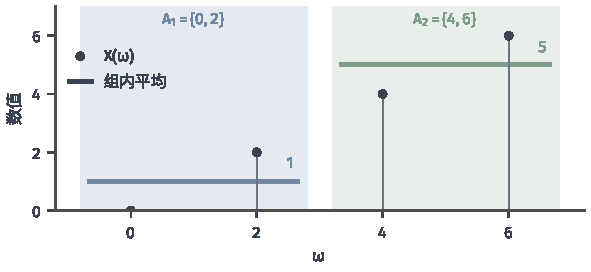
\includegraphics[width=100mm]{figures/02-abstract-mathematics/02-probability-spaces/matplotlib/cond-four-points/figure.pdf}
  \caption{四点空间上的分组平均。样本空间$\Omega=\{0,2,4,6\}$，每点概率$1/4$，圆点和竖线给出$X(\omega)=\omega$。蓝色与绿色底色分别是只能辨认的两组$A_1=\{0,2\}$和$A_2=\{4,6\}$，粗横线是组内平均$1$和$5$，它们合起来就是条件平均$Z$。}
  \label{fig:cond-four-points}
\end{figure}

\paragraph{条件平均保留的两项性质}
$Z$有两项性质值得单独写出。
第一，$Z$在每一块上取常值，因此只要知道样本点落在哪一块，就能确定$Z$的值；它只使用分组信息。
第二，在每一块上，$Z$与$X$的积分总量相同：
\[
  \mathbb E[Z\mathbb I_{A_i}]=\frac{\mathbb E[X\mathbb I_{A_i}]}{\mathbb P(A_i)}\,\mathbb P(A_i)=\mathbb E[X\mathbb I_{A_i}].
\]
在示例~\ref{ex:cond-four-points}中，两边分别是$1\times\frac12=\frac12$与$\frac{0+2}{4}=\frac12$。

观察者能够判断是否发生的事件，不只是单独的块，还有若干块的并。
由于积分对不交并可加，第二项性质对任意若干块的并同样成立；取全部块的并$\Omega$，得到$\mathbb EZ=\mathbb EX$，在示例中两边都是$3$。
这两项性质——只依赖可用信息、在每个可观察事件上保持积分——就是下一节抽象定义要保留的全部内容。

还有一个细节。
若某块$A_i$的概率为零，式~\eqref{eq:cond-group-average}无法计算；但无论在$A_i$上给$Z$赋什么值，$\mathbb E[Z\mathbb I_A]$对任何事件$A$都不变。
因此零概率分组上的赋值不影响上述两项性质，我们暂不为它规定唯一答案。

\subsection{子$\sigma$代数与可用信息}

\paragraph{用子$\sigma$代数表示可辨认的事件}
第~\ref{chap:probability-models}章用生成$\sigma$代数$\sigma(Y)$（定义~\ref{def:pmod-generated-sigma}）记录观测$Y$能够回答的全部“是否发生”问题。
一般地，我们用子$\sigma$代数$\mathcal G\subseteq\mathcal F$表示允许辨认的事件：$A\in\mathcal G$意味着观察者能判断$A$是否发生。
对$\mathcal G$可测的随机变量，其每个水平事件$\{Z\leq c\}$都在$\mathcal G$中，因而可以完全依据这些信息确定。
在有限划分的情形，$\mathcal G$由各块的全部并组成，$\mathcal G$可测恰好意味着在每一块上取常值，这正是上一小节的第一项性质。

信息的多少由事件族的包含关系衡量，而不是由观测的维数衡量。
若$\mathcal H\subseteq\mathcal G$，凡是用$\mathcal H$能判断的事件用$\mathcal G$也能判断，我们说$\mathcal G$比$\mathcal H$含有更多信息。
二维观测$(Y,2Y)$与一维观测$Y$生成同一个$\sigma$代数，因此信息相同；反过来，在$\Omega=[0,1)$（取$\mathcal F$为Borel $\sigma$代数）上，一维的恒等映射$\omega\mapsto\omega$就生成全部Borel事件，已经是完全信息。

图~\ref{fig:cond-information-layers}在$\Omega=[0,1)$（概率为长度）上比较四个逐步加细的信息。
取$X(\omega)=2\omega+\sin(2\pi\omega)$。
只知道“某事发生了”时，最好的平均只能是常数$\mathbb EX=1$；把区间分成两块、四块后，组内平均变成两级、四级阶梯；完全信息下，条件平均就是$X$本身。
信息越细，阶梯越贴近原函数，但每一级阶梯始终只依赖当前能辨认的块。

\begin{figure*}[htbp]
  \centering
  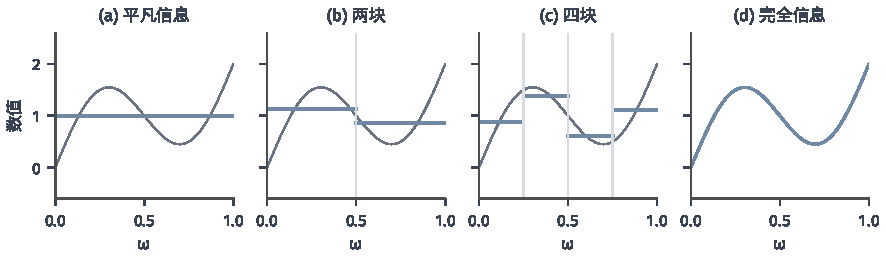
\includegraphics[width=150mm]{figures/02-abstract-mathematics/02-probability-spaces/matplotlib/cond-information-layers/figure.pdf}
  \caption{四种信息下的条件平均。样本空间为$[0,1)$，概率为长度；灰线是$X(\omega)=2\omega+\sin(2\pi\omega)$，蓝线是给定信息下的条件平均。(a)平凡信息，条件平均为常数$\mathbb EX=1$；(b)按$[0,\frac12),[\frac12,1)$分组，组内平均约为$1.137,0.863$；(c)按四个等长区间分组，组内平均约为$0.887,1.387,0.613,1.113$；(d)完全信息，条件平均与$X$重合。组内平均用$200000$个中点格点数值积分得到。}
  \label{fig:cond-information-layers}
\end{figure*}

\paragraph{两个极端与连续观测的困难}
两个极端情形可以直接从两项性质读出答案。
平凡$\sigma$代数$\{\varnothing,\Omega\}$只允许判断“某事发生了”，对它可测的随机变量只有常数；在$A=\Omega$上保持积分，要求这个常数等于$\mathbb EX$。
另一端$\mathcal G=\mathcal F$允许辨认全部事件，$X$本身就满足两项性质，条件平均应当是$X$。

有限划分的做法却不能直接搬到连续观测。
若$Y$服从标准正态分布，每个$\{Y=y\}$的概率都是零，式~\eqref{eq:cond-group-average}的分母为零；而$\sigma(Y)$中的事件$\{Y\in B\}$有不可数多个，也不能把它们看成有限个块的并。
于是自然的问题是：能否只保留“对$\mathcal G$可测”和“在$\mathcal G$的每个事件上保持积分”这两项要求，而完全不做逐组除法？
下一节说明这样做不仅可行，而且结果几乎处处唯一。

\section{条件期望的定义与存在性}
\label{sec:cond-definition}

本节固定概率空间$(\Omega,\mathcal F,\mathbb P)$与子$\sigma$代数$\mathcal G\subseteq\mathcal F$。
我们先把上一节的两项要求写成定义，再用Radon--Nikodym定理证明满足要求的随机变量存在，最后把抽象的信息$\mathcal G$换回具体的观测$Y$。

\subsection{条件期望的定义}

\paragraph{两项要求的一般形式}
上一节的两项性质不涉及除法，可以原样推广到任意子$\sigma$代数。

\begin{definition}[条件期望]
\label{def:cond-expectation}
设$X$是可积的实值随机变量，$\mathcal G\subseteq\mathcal F$是子$\sigma$代数。
若可积随机变量$Z$满足
\begin{enumerate}
  \item $Z$对$\mathcal G$可测；
  \item 对每个$A\in\mathcal G$，
  \begin{equation}
    \mathbb E[Z\mathbb I_A]=\mathbb E[X\mathbb I_A],
    \label{eq:cond-defining-identity}
  \end{equation}
\end{enumerate}
则称$Z$为$X$给定$\mathcal G$的\term{条件期望}（conditional expectation），记作$\mathbb E[X\mid\mathcal G]$。
\end{definition}

第一项条件说$Z$只使用$\mathcal G$中的信息，第二项条件说在每个可以观察的事件上，$Z$与$X$有相同的积分总量。
对有限划分生成的$\mathcal G$，上一节已经验证分组平均满足这两项条件：$\mathcal G$中的事件是若干块的并，而式~\eqref{eq:cond-defining-identity}对每一块成立，从而对它们的不交并也成立。
因此示例~\ref{ex:cond-four-points}中的$Z$就是$\mathbb E[X\mid\mathcal G]$，其中$\mathcal G=\{\varnothing,A_1,A_2,\Omega\}$。

\paragraph{版本与条件概率}
条件期望是一个随机变量，而不是一个数。
下一小节将证明，满足定义的两个随机变量几乎必然相等（几乎必然的含义见定义~\ref{def:pmod-almost-sure}）；反过来，在$\mathcal G$中的零概率事件上改动$Z$，两项条件仍然成立。
所以定义确定的是一个几乎处处等价类，其中每一个具体的随机变量称为条件期望的一个版本。
写$\mathbb E[X\mid\mathcal G]=W$时，意思是$W$是一个版本；涉及条件期望的等式和不等式，默认都在几乎必然意义下成立。

取$X=\mathbb I_B$（$B\in\mathcal F$），就得到事件的条件概率
\[
  \mathbb P(B\mid\mathcal G)=\mathbb E[\mathbb I_B\mid\mathcal G].
\]
它满足$\mathbb E[\mathbb P(B\mid\mathcal G)\mathbb I_A]=\mathbb P(A\cap B)$对每个$A\in\mathcal G$成立，这正是“组内频率乘以组的概率等于交事件概率”的一般形式。
对有限维可积随机向量$\bm X=(X_1,\ldots,X_d)$，逐坐标定义$\mathbb E[\bm X\mid\mathcal G]$即可。
一般取值空间中的随机对象不一定能求平均，例如取值于一个没有线性结构的集合；它们的条件规律要用第~\ref{sec:cond-distributions}节的条件分布描述。

\subsection{条件期望的存在性与唯一性}

\paragraph{把积分总量看成测度}
定义只说了条件期望应当满足什么，还没有说明这样的随机变量一定存在。
关键的观察是：等式~\eqref{eq:cond-defining-identity}的右边$A\mapsto\mathbb E[X\mathbb I_A]$在$X\geq0$时是$\mathcal G$上的一个有限测度，而左边要求它由某个$\mathcal G$可测函数作为密度给出。
这正是Radon--Nikodym定理（定理~\ref{thm:density-radon-nikodym}）回答的问题：若$\sigma$有限测度$\nu$关于$\sigma$有限测度$\mu$绝对连续，则存在非负可测函数$f$使$\nu(A)=\int_Af\,d\mu$对每个可测集$A$成立。

需要注意的是，这里两个测度都只定义在$\mathcal G$上。
$X$本身一般不对$\mathcal G$可测，因此$X$不是所求的密度；密度定理在较小的$\sigma$代数上重新寻找一个$\mathcal G$可测的密度，这一步正是“只用可用信息”的数学体现。

\begin{theorem}[条件期望的存在性与唯一性]
\label{thm:cond-existence}
设$X$是可积随机变量，$\mathcal G\subseteq\mathcal F$是任意子$\sigma$代数。
则$\mathbb E[X\mid\mathcal G]$存在；若$Z_1,Z_2$都满足定义~\ref{def:cond-expectation}，则$Z_1=Z_2$几乎必然成立。
\end{theorem}

\begin{proof}
\emph{非负情形的存在性。}
先设$X\geq0$。在可测空间$(\Omega,\mathcal G)$上定义
\[
  \nu(A)=\mathbb E[X\mathbb I_A],\qquad A\in\mathcal G.
\]
若$A_1,A_2,\ldots\in\mathcal G$两两不交，则$\mathbb I_{\bigcup_kA_k}=\sum_k\mathbb I_{A_k}$，对非负部分和用单调收敛定理得$\nu(\bigcup_kA_k)=\sum_k\nu(A_k)$；又$\nu(\Omega)=\mathbb EX<\infty$，所以$\nu$是有限测度。
记$\mathbb P|_{\mathcal G}$为$\mathbb P$在$\mathcal G$上的限制，它是$(\Omega,\mathcal G)$上的概率测度。
若$A\in\mathcal G$且$\mathbb P(A)=0$，则非负随机变量$X\mathbb I_A$几乎必然为零，故$\nu(A)=0$；这说明$\nu\ll\mathbb P|_{\mathcal G}$。
两个测度都有限，由Radon--Nikodym定理，存在$\mathcal G$可测的非负函数$Z$，使
\[
  \nu(A)=\int_AZ\,d\mathbb P|_{\mathcal G},\qquad A\in\mathcal G.
\]
对$\mathcal G$可测的非负函数，关于$\mathbb P|_{\mathcal G}$与关于$\mathbb P$的积分相同：两者在$\mathcal G$中事件的示性函数上一致，从而在$\mathcal G$可测简单函数上一致，再由单调收敛推广到非负$\mathcal G$可测函数。
于是$\mathbb E[Z\mathbb I_A]=\mathbb E[X\mathbb I_A]$对每个$A\in\mathcal G$成立。取$A=\Omega$得$\mathbb EZ=\mathbb EX<\infty$，所以$Z$可积，它满足定义~\ref{def:cond-expectation}。

\emph{一般情形的存在性。}
对一般可积$X$，写$X=X^+-X^-$，其中$X^+=\max(X,0)$、$X^-=\max(-X,0)$都非负可积。
由上一步分别得到$Z^+=\mathbb E[X^+\mid\mathcal G]$与$Z^-=\mathbb E[X^-\mid\mathcal G]$，令$Z=Z^+-Z^-$。
$Z$对$\mathcal G$可测且可积，并且对每个$A\in\mathcal G$，
\[
  \mathbb E[Z\mathbb I_A]=\mathbb E[Z^+\mathbb I_A]-\mathbb E[Z^-\mathbb I_A]=\mathbb E[X^+\mathbb I_A]-\mathbb E[X^-\mathbb I_A]=\mathbb E[X\mathbb I_A].
\]
这里先拆开正负部分，是因为有符号的$A\mapsto\mathbb E[X\mathbb I_A]$不是非负测度，不能直接套用密度定理。

\emph{唯一性。}
设$Z_1,Z_2$都满足定义。事件$A=\{Z_1>Z_2\}$由两个$\mathcal G$可测函数确定，所以$A\in\mathcal G$。由式~\eqref{eq:cond-defining-identity}，
\[
  \mathbb E[(Z_1-Z_2)\mathbb I_A]=\mathbb E[X\mathbb I_A]-\mathbb E[X\mathbb I_A]=0.
\]
被积函数$(Z_1-Z_2)\mathbb I_A$非负且积分为零，因而几乎必然为零；而它在$A$上严格为正，所以$\mathbb P(A)=0$。
交换$Z_1,Z_2$的角色得$\mathbb P(Z_2>Z_1)=0$，故$Z_1=Z_2$几乎必然成立。
\end{proof}

\paragraph{这一论证不需要的条件}
证明对$\mathcal G$没有任何额外要求：它不必由可数个事件生成，样本空间也不必是标准Borel空间。
用到的只有两点：$\mathcal G$上的有限测度可以用密度表示，以及$\{Z_1>Z_2\}$这类事件本身就在$\mathcal G$中。
后面把全部事件的条件概率组织成一个分布时，空间结构的条件才会出现；那是另一个问题，不影响逐个可积变量的条件期望。

\paragraph{只在生成族上检验}
实际验证某个$W$是条件期望时，$\mathcal G$中的事件往往太多，无法逐个检查。
下面的引理说明，只需在一个对有限交封闭、且包含$\Omega$的生成族上检验等式~\eqref{eq:cond-defining-identity}。

\begin{lemma}[生成族上的检验]
\label{lem:cond-pi-check}
设$X$可积，$W$可积且对$\mathcal G$可测。若$\mathcal C$是生成$\mathcal G$的$\pi$系统，$\Omega\in\mathcal C$，并且$\mathbb E[W\mathbb I_C]=\mathbb E[X\mathbb I_C]$对每个$C\in\mathcal C$成立，则$W=\mathbb E[X\mid\mathcal G]$。
\end{lemma}

\begin{proof}
令$\mathcal D=\{A\in\mathcal G:\mathbb E[W\mathbb I_A]=\mathbb E[X\mathbb I_A]\}$，则$\mathcal C\subseteq\mathcal D$。
若$A\in\mathcal D$，由$\Omega\in\mathcal D$及$\mathbb I_{A^c}=1-\mathbb I_A$得$A^c\in\mathcal D$。
若$A_1,A_2,\ldots\in\mathcal D$两两不交，记$A=\bigcup_kA_k$，则$\sum_{k\leq n}W\mathbb I_{A_k}\to W\mathbb I_A$，且绝对值被可积的$|W|$控制，由控制收敛定理和$X$的同样论证得$A\in\mathcal D$。
因此$\mathcal D$对补集和不交可数并封闭。由$\pi$--$\lambda$定理（定理~\ref{thm:measure-pi-lambda}），包含$\pi$系统$\mathcal C$的这类集合族必包含$\sigma(\mathcal C)=\mathcal G$。
\end{proof}

\subsection{给定随机变量的条件期望}

\paragraph{观测值上的函数}
实际问题中的信息通常来自一个观测$Y$，它取值于可测空间$(E,\mathcal E)$。
我们定义
\[
  \mathbb E[X\mid Y]=\mathbb E[X\mid\sigma(Y)].
\]
它是$\sigma(Y)$可测的随机变量。
为了说出“给定$Y=y$时的平均”，需要把这样的随机变量写成观测值的函数；下面的结论通常称为\term{Doob--Dynkin引理}。

\begin{theorem}[Doob--Dynkin引理]
\label{thm:cond-doob-dynkin}
设$Y$取值于可测空间$(E,\mathcal E)$，$Z$是实值随机变量。
则$Z$对$\sigma(Y)$可测，当且仅当存在可测函数$h:E\to\mathbb R$，使$Z=h(Y)$在$\Omega$上处处成立。
\end{theorem}

\begin{proof}
若$Z=h(Y)$，则对每个Borel集$B$，$\{Z\in B\}=\{Y\in h^{-1}(B)\}\in\sigma(Y)$，所以$Z$对$\sigma(Y)$可测。

反过来，先设$Z=\mathbb I_A$，$A\in\sigma(Y)$。由$\sigma(Y)=\{\{Y\in B\}:B\in\mathcal E\}$，存在$B\in\mathcal E$使$A=\{Y\in B\}$，于是$Z=\mathbb I_B(Y)$。
对$\sigma(Y)$可测的简单函数$Z=\sum_ka_k\mathbb I_{A_k}$，逐项使用上一步并取线性组合即可。
对一般实值$\sigma(Y)$可测的$Z$，取$\sigma(Y)$可测简单函数$Z_n$逐点收敛到$Z$，并写$Z_n=h_n(Y)$。
令$L=\{y\in E:\lim_nh_n(y)\text{存在且有限}\}$，它由可数个可测函数的上、下极限确定，因而属于$\mathcal E$；定义$h(y)=\lim_nh_n(y)$（$y\in L$），在$L$外令$h(y)=0$，则$h$可测。
对每个$\omega$，$h_n(Y(\omega))=Z_n(\omega)\to Z(\omega)$，所以$Y(\omega)\in L$且$h(Y(\omega))=Z(\omega)$。
\end{proof}

证明中把$h$在$L$外补成零，是因为$h_n$只在$Y$实际取到的值上被$Z_n$约束，别处可能不收敛。
将定理用于$Z=\mathbb E[X\mid Y]$，得到可测函数$h$使$\mathbb E[X\mid Y]=h(Y)$，我们记
\[
  \mathbb E[X\mid Y=y]=h(y).
\]
这样，“给定$Y=y$后的条件平均”就有了准确含义：它是观测值上的一个函数，由积分条件
\begin{equation}
  \mathbb E[X\mathbb I_{\{Y\in B\}}]=\int_Bh(y)\,P_Y(dy),\qquad B\in\mathcal E
  \label{eq:cond-given-y-identity}
\end{equation}
刻画，右边用的是$Y$的分布$P_Y$和换元公式（定理~\ref{thm:pmod-change-of-variables}）。

$h$只在$P_Y$几乎处处的意义下确定。
若$h(Y)$与$h'(Y)$都是$\mathbb E[X\mid Y]$的版本，则$P_Y(\{h\neq h'\})=\mathbb P(h(Y)\neq h'(Y))=0$；反之，在一个$P_Y$零集上改动$h$，$h(Y)$只在一个零概率事件上改变，仍是一个版本。

\paragraph{离散观测与连续观测}
若$Y$只取有限个值$y_1,\ldots,y_m$，且每个$\mathbb P(Y=y_j)>0$，在式~\eqref{eq:cond-given-y-identity}中取$B=\{y_j\}$，得
\[
  h(y_j)=\frac{\mathbb E[X\mathbb I_{\{Y=y_j\}}]}{\mathbb P(Y=y_j)},
\]
这就回到第~\ref{sec:cond-information}节的分组平均，划分由$\{Y=y_j\}$给出。
卷一已经用这种按值分组的方式和普通密度计算过条件均值与全期望公式，本章的定义把那里的计算放进同一个框架，可参考\BookChapterRef{chap:random-vectors}{卷一“随机向量与联合分布”章}。

连续观测下，式~\eqref{eq:cond-given-y-identity}同样有意义，但它只约束$h$在$P_Y$意义下的“几乎所有”取值。
若$(X,Y)$有联合密度$p(x,y)$，在$0<p_Y(y)<\infty$且$\int|x|\,p(x,y)\,dx<\infty$处令$h(y)=\int x\,p(x,y)\,dx/p_Y(y)$，其余$y$处令$h(y)=0$。由$X$可积和Tonelli定理，被排除的$y$构成$P_Y$零集；再用Fubini定理可以验证$h$满足式~\eqref{eq:cond-given-y-identity}，因而是一个方便计算的版本。
但条件期望的定义与存在都不依赖联合密度，也从不把$\mathbb P(Y=y)=0$处的平均解释为两个零的比值。

\begin{example}[平方关系加独立噪声]
\label{ex:cond-square-noise}
设$Y\sim N(0,1)$，$\varepsilon\sim N(0,\sigma^2)$与$Y$独立，$X=Y^2+\varepsilon$。
我们直接用定义验证$h(y)=y^2$。
$h(Y)=Y^2$对$\sigma(Y)$可测且可积。对每个Borel集$B$，
\[
  \begin{aligned}
  \mathbb E[X\mathbb I_{\{Y\in B\}}]&=\mathbb E[Y^2\mathbb I_B(Y)]+\mathbb E[\varepsilon\,\mathbb I_B(Y)]\\
  &=\mathbb E[Y^2\mathbb I_B(Y)]+\mathbb E\varepsilon\cdot\mathbb P(Y\in B)=\mathbb E[Y^2\mathbb I_B(Y)],
  \end{aligned}
\]
第二个等号用了独立可积变量乘积的期望等于期望之积（定理~\ref{thm:pmod-product-expectation}）。
所以$\mathbb E[X\mid Y]=Y^2$，即$\mathbb E[X\mid Y=y]=y^2$。
\end{example}

图~\ref{fig:cond-regression-scatter}取$\sigma=0.5$，画出$600$个样本点$(Y,X)$。
如果把$Y$的取值范围切成宽$0.5$的小段，每一段就是一个正概率的组，组内平均（绿色短横线）是给定“$Y$落在哪一段”这一较粗信息的条件平均的经验估计。
这些短横线紧贴红色曲线$h(y)=y^2$。
不过要注意二者的关系：$h$不是由“分段越来越细”的极限定义的，而是由式~\eqref{eq:cond-given-y-identity}直接刻画；分段平均只是更粗信息下的条件平均，第~\ref{sec:cond-properties}节的塔式法则将说明它等于$h(Y)$在段内的平均。

\begin{figure}[htbp]
  \centering
  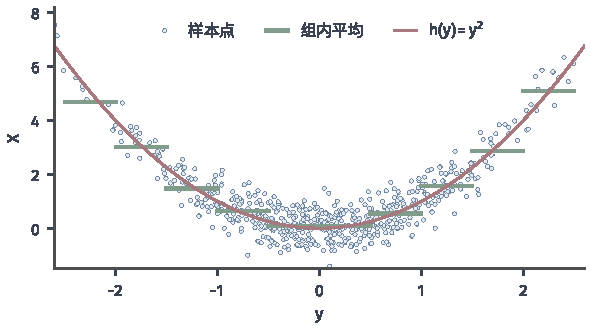
\includegraphics[width=100mm]{figures/02-abstract-mathematics/02-probability-spaces/matplotlib/cond-regression-scatter/figure.pdf}
  \caption{连续观测下的条件期望$\mathbb E[X\mid Y=y]=h(y)$。模型为$Y\sim N(0,1)$，$\varepsilon\sim N(0,0.25)$与$Y$独立，$X=Y^2+\varepsilon$；圆点为固定随机种子生成的$600$个样本，红线为$h(y)=y^2$，绿色短横线为$Y$按宽$0.5$分段后各段（至少含$5$个样本）的组内平均。}
  \label{fig:cond-regression-scatter}
\end{figure}

\section{条件期望的性质}
\label{sec:cond-properties}

有了定义和存在唯一性，我们分别研究条件期望的代数运算、信息嵌套、误差比较与极限交换。
各项性质的证明都回到同一个判定方法：先说明候选随机变量对当前信息可测，再检验它在可观察事件上的积分；唯一性（定理~\ref{thm:cond-existence}）随后保证它就是条件期望。

\subsection{条件期望的运算规则}

\paragraph{线性、保序与可测量保持}
组内平均对被平均的量是线性的：两个变量之和的组内平均等于各自组内平均之和；它也不会把逐点较小的量平均成较大的量。
下面的定理说明这些直观规则在一般情形下仍然成立，只是都附带“几乎必然”。

\begin{theorem}[条件期望的基本运算规则]
\label{thm:cond-rules}
设$X,X'$可积，$a,b\in\mathbb R$，$\mathcal G\subseteq\mathcal F$是子$\sigma$代数。则以下各式几乎必然成立：
\begin{enumerate}
  \item 线性：$\mathbb E[aX+bX'\mid\mathcal G]=a\,\mathbb E[X\mid\mathcal G]+b\,\mathbb E[X'\mid\mathcal G]$；
  \item 保序：若$X\leq X'$几乎必然成立，则$\mathbb E[X\mid\mathcal G]\leq\mathbb E[X'\mid\mathcal G]$；
  \item 可测量保持：若$X$对$\mathcal G$可测，则$\mathbb E[X\mid\mathcal G]=X$；特别地，常数$c$满足$\mathbb E[c\mid\mathcal G]=c$；
  \item 绝对值：$\bigl|\mathbb E[X\mid\mathcal G]\bigr|\leq\mathbb E[|X|\mid\mathcal G]$；
  \item 总平均：$\mathbb E\bigl[\mathbb E[X\mid\mathcal G]\bigr]=\mathbb EX$。
\end{enumerate}
\end{theorem}

\begin{proof}
记$Z=\mathbb E[X\mid\mathcal G]$，$Z'=\mathbb E[X'\mid\mathcal G]$。
(1) $aZ+bZ'$对$\mathcal G$可测且可积，对每个$A\in\mathcal G$有$\mathbb E[(aZ+bZ')\mathbb I_A]=a\mathbb E[X\mathbb I_A]+b\mathbb E[X'\mathbb I_A]=\mathbb E[(aX+bX')\mathbb I_A]$，由唯一性得结论。
(2) 由(1)，$W=Z'-Z$是$X'-X$的条件期望。令$A=\{W<0\}\in\mathcal G$，则$\mathbb E[W\mathbb I_A]=\mathbb E[(X'-X)\mathbb I_A]\geq0$；而$W\mathbb I_A\leq0$，故$W\mathbb I_A=0$几乎必然成立，这只能在$\mathbb P(A)=0$时发生。
(3) 此时$X$本身满足定义的两项条件。
(4) 由$-|X|\leq X\leq|X|$和(1)(2)得$-\mathbb E[|X|\mid\mathcal G]\leq Z\leq\mathbb E[|X|\mid\mathcal G]$。
(5) 在式~\eqref{eq:cond-defining-identity}中取$A=\Omega$。
\end{proof}

回到示例~\ref{ex:cond-four-points}检查这些规则的含义。
$\mathbb E[X+2\mid\mathcal G]$在两组上取$3,7$，正是$1,5$各加$2$。
绝对值规则中的不等号可以是严格的：对$X-1$，它在四点上取$-1,1,3,5$，条件期望在两组上为$0,4$；而$|X-1|$取$1,1,3,5$，条件期望为$1,4$。
第一组内$-1$与$1$相互抵消，所以先平均再取绝对值得到$0$，比先取绝对值再平均的$1$小。

\paragraph{提出已知因子}
若$H$对$\mathcal G$可测，那么在观察者眼中$H$的值是已知的，计算$HX$的条件平均时应当可以把它当作常数提出。
这一直观需要可积性条件来保证。

\begin{theorem}[提出已知因子]
\label{thm:cond-pull-out}
设$H$对$\mathcal G$可测，$X$与$HX$都可积。则$H\,\mathbb E[X\mid\mathcal G]$可积，并且
\[
  \mathbb E[HX\mid\mathcal G]=H\,\mathbb E[X\mid\mathcal G]\qquad\text{几乎必然}.
\]
\end{theorem}

\begin{proof}
记$Z=\mathbb E[X\mid\mathcal G]$。由于$HZ$对$\mathcal G$可测，只需在可积性成立后验证$\mathbb E[HZ\mathbb I_A]=\mathbb E[HX\mathbb I_A]$对每个$A\in\mathcal G$成立。

\emph{有界乘子。}若$H=\mathbb I_B$，$B\in\mathcal G$，则$A\cap B\in\mathcal G$，于是
$\mathbb E[\mathbb I_BZ\mathbb I_A]=\mathbb E[Z\mathbb I_{A\cap B}]=\mathbb E[X\mathbb I_{A\cap B}]=\mathbb E[\mathbb I_BX\mathbb I_A]$。
由线性，等式对$\mathcal G$可测的简单函数$H$成立。
若$|H|\leq c$，取$\mathcal G$可测简单函数$H_n\to H$逐点且$|H_n|\leq c$；两边的被积函数分别被可积的$c|Z|$与$c|X|$控制，由控制收敛定理，等式对$H$成立。

\emph{非负因子的截断。}设$H\geq0$、$X\geq0$，则$Z\geq0$几乎必然成立（定理~\ref{thm:cond-rules}）。截断$H\wedge n$有界，所以
$\mathbb E[(H\wedge n)Z\mathbb I_A]=\mathbb E[(H\wedge n)X\mathbb I_A]$。令$n\to\infty$，两边被积函数单调上升，由单调收敛定理得$\mathbb E[HZ\mathbb I_A]=\mathbb E[HX\mathbb I_A]$；取$A=\Omega$知$\mathbb E[HZ]=\mathbb E[HX]<\infty$，故$HZ$可积。

\emph{一般情形。}写$H=H^+-H^-$，$X=X^+-X^-$。四个乘积$H^\pm X^\pm$都不超过$|HX|$，因而可积，上一步给出$\mathbb E[H^\pm X^\pm\mid\mathcal G]=H^\pm\,\mathbb E[X^\pm\mid\mathcal G]$，且右边可积。
由$HX=H^+X^+-H^+X^--H^-X^++H^-X^-$与线性，
\[
  \mathbb E[HX\mid\mathcal G]=(H^+-H^-)\bigl(\mathbb E[X^+\mid\mathcal G]-\mathbb E[X^-\mid\mathcal G]\bigr)=HZ.
\]
\end{proof}

定理要求的是$X$与$HX$可积，而不是只要求$X$可积。
首先，$HX$可积才使左边的$\mathbb E[HX\mid\mathcal G]$在定义~\ref{def:cond-expectation}的意义下有意义；其次，截断步骤里的单调收敛本身允许极限为$+\infty$，正是$\mathbb E[HX]<\infty$才推出$HZ$可积，一般情形把四个部分相减时也才不会出现$\infty-\infty$。

被提出的因子必须对$\mathcal G$可测，依赖组内未观察信息的乘子不能提出。
在示例~\ref{ex:cond-four-points}中取$H=X$，它不对$\mathcal G$可测：
$\mathbb E[X\cdot X\mid\mathcal G]$在两组上为$\frac{0+4}{2}=2$与$\frac{16+36}{2}=26$，而$X\,\mathbb E[X\mid\mathcal G]$在四点上取$0,2,20,30$，连对$\mathcal G$可测都不满足。
若提出的是已知的$\mathbb E[X\mid\mathcal G]$，得到$\mathbb E[X\mid\mathcal G]^2$，在两组上为$1,25$；它与$2,26$的差恰为组内方差$1$。

\subsection{嵌套信息与塔式法则}

\paragraph{两种嵌套顺序}
设$\mathcal H\subseteq\mathcal G$，也就是说$\mathcal G$比$\mathcal H$含有更多信息。
先在较细的信息$\mathcal G$下求平均，再在较粗的信息$\mathcal H$下求平均，结果应当与直接在$\mathcal H$下求平均相同；这就是分组平均中“先求小组平均，再按小组大小合并”的一般形式。

\begin{theorem}[塔式法则]
\label{thm:cond-tower}
设$X$可积，$\mathcal H\subseteq\mathcal G\subseteq\mathcal F$都是子$\sigma$代数。则几乎必然有
\[
  \mathbb E\bigl[\mathbb E[X\mid\mathcal G]\bigm|\mathcal H\bigr]=\mathbb E[X\mid\mathcal H],\qquad
  \mathbb E\bigl[\mathbb E[X\mid\mathcal H]\bigm|\mathcal G\bigr]=\mathbb E[X\mid\mathcal H].
\]
\end{theorem}

\begin{proof}
记$Z=\mathbb E[X\mid\mathcal G]$，$W=\mathbb E[X\mid\mathcal H]$。
第一式：$W$对$\mathcal H$可测且可积。对每个$A\in\mathcal H$，由于$A$也属于$\mathcal G$，两次使用定义得
$\mathbb E[Z\mathbb I_A]=\mathbb E[X\mathbb I_A]=\mathbb E[W\mathbb I_A]$，所以$W$满足$Z$给定$\mathcal H$的条件期望的定义。
第二式：$W$对$\mathcal H$可测，因而对更大的$\mathcal G$也可测，由定理~\ref{thm:cond-rules}的可测量保持，$\mathbb E[W\mid\mathcal G]=W$。
\end{proof}

两式的理由不同。
第一式用的是“粗信息下的事件也是细信息下的事件”，所以细平均在粗事件上的总量与原变量相同；第二式用的是“粗平均已经只依赖粗信息，再给它更多信息也不会改变”。
两种顺序最终都落在较粗的信息上，这是$\mathcal H\subseteq\mathcal G$带来的。
这一结论通常称为\term{塔式法则}（tower property）。

\paragraph{全期望公式与独立信息}
取$\mathcal H=\{\varnothing,\Omega\}$，对它的条件期望就是常数期望，塔式法则成为
\[
  \mathbb E\bigl[\mathbb E[X\mid\mathcal G]\bigr]=\mathbb EX,
\]
即全期望公式；它与定理~\ref{thm:cond-rules}的第五条一致。

另一个常用的特例是$X$与$\mathcal G$独立，即$\sigma(X)$与$\mathcal G$独立（定义~\ref{def:pmod-independence}）。
这时观察$\mathcal G$对$X$没有任何帮助，条件期望应当退化为常数$\mathbb EX$。
验证如下：常数$\mathbb EX$对$\mathcal G$可测；对每个$A\in\mathcal G$，$X$与$\mathbb I_A$独立且都可积，由定理~\ref{thm:pmod-product-expectation}，
\[
  \mathbb E[X\mathbb I_A]=\mathbb EX\cdot\mathbb P(A)=\mathbb E[(\mathbb EX)\mathbb I_A].
\]
所以$\mathbb E[X\mid\mathcal G]=\mathbb EX$。示例~\ref{ex:cond-square-noise}中$\mathbb E[\varepsilon\mid Y]=\mathbb E\varepsilon=0$正是这种情形。

\paragraph{粗细两层分组的计算}
图~\ref{fig:cond-tower-layers}用八个等概率样本点展示塔式法则。
$X$在八点上依次取$1,3,2,6,5,9,4,8$。
细信息$\mathcal G$把相邻两点分为一组，组内平均为$2,4,7,6$；粗信息$\mathcal H$把前四点和后四点各分为一组，组内平均为$3$与$6.5$。
在粗组内平均细平均，$(2+4)/2=3$，$(7+6)/2=6.5$，与直接在粗组内平均原数据相同；再平均一次得到$\mathbb EX=4.75$。
每一层只需要上一层的结果，不需要回到原始数据，这正是塔式法则在计算中的用途。

\begin{figure}[htbp]
  \centering
  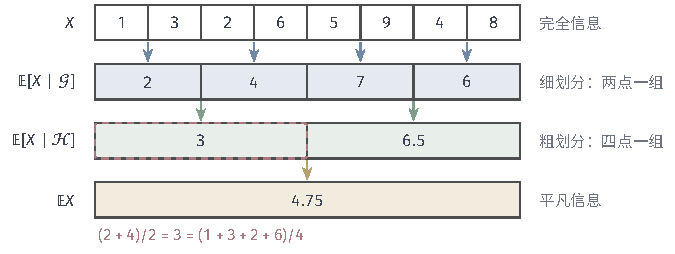
\includegraphics[width=112mm]{figures/02-abstract-mathematics/02-probability-spaces/tikz/cond-tower-layers/figure.pdf}
  \caption{塔式法则的逐层平均。八个样本点等概率，第一行是$X$的取值；第二行按相邻两点分组（信息$\mathcal G$），第三行按前后四点分组（信息$\mathcal H\subseteq\mathcal G$），第四行为平凡信息下的$\mathbb EX$。箭头表示在下一层的组内平均上一层；红色虚线框标出第一个粗组，图下方的红色算式说明在该组内先细后粗与直接粗分组的结果相同。}
  \label{fig:cond-tower-layers}
\end{figure}

两个没有包含关系的$\sigma$代数不能直接套用塔式法则。
在示例~\ref{ex:cond-four-points}的四点空间上，令$\mathcal G_1$由$\{0,2\},\{4,6\}$生成，$\mathcal G_2$由$\{0\},\{2,4,6\}$生成。
$\mathbb E[X\mid\mathcal G_1]$在四点上取$1,1,5,5$，$\mathbb E[X\mid\mathcal G_2]$取$0,4,4,4$。
再交换条件化：$\mathbb E\bigl[\mathbb E[X\mid\mathcal G_1]\bigm|\mathcal G_2\bigr]$取$1,\frac{11}{3},\frac{11}{3},\frac{11}{3}$，$\mathbb E\bigl[\mathbb E[X\mid\mathcal G_2]\bigm|\mathcal G_1\bigr]$取$2,2,4,4$。
两种顺序结果不同，而$\mathcal G_1\cap\mathcal G_2$是平凡$\sigma$代数，对它的条件期望是常数$3$，与两者都不相同。

\subsection{条件平均与误差控制}

\paragraph{条件Jensen不等式}
第~\ref{chap:probability-models}章的Jensen不等式（定理~\ref{thm:pmod-jensen}）说，对凸函数$\varphi$，先平均再作用不超过先作用再平均：$\varphi(\mathbb EX)\leq\mathbb E\varphi(X)$。
在每个组内做同样的比较，就得到它的条件版本。

\begin{theorem}[条件Jensen不等式]
\label{thm:cond-jensen}
设$\varphi:\mathbb R\to\mathbb R$是凸函数，$X$与$\varphi(X)$都可积。则
\[
  \varphi\bigl(\mathbb E[X\mid\mathcal G]\bigr)\leq\mathbb E[\varphi(X)\mid\mathcal G]\qquad\text{几乎必然}.
\]
\end{theorem}

\begin{proof}
凸函数在每点有有限的右导数$\varphi'_+(q)$，并且直线$\ell_q(x)=\varphi(q)+\varphi'_+(q)(x-q)$处处位于$\varphi$下方。
我们断言$\varphi(x)=\sup_{q\in\mathbb Q}\ell_q(x)$对每个$x$成立。
“$\geq$”由支撑性质得到；对“$\leq$”，取有理数$q_k\to x$，凸函数连续且右导数在$x$附近有界，所以$\ell_{q_k}(x)=\varphi(q_k)+\varphi'_+(q_k)(x-q_k)\to\varphi(x)$。
对每个有理数$q$，由$\ell_q(X)\leq\varphi(X)$以及定理~\ref{thm:cond-rules}的线性与保序，
\[
  \ell_q\bigl(\mathbb E[X\mid\mathcal G]\bigr)=\varphi(q)+\varphi'_+(q)\bigl(\mathbb E[X\mid\mathcal G]-q\bigr)\leq\mathbb E[\varphi(X)\mid\mathcal G]
\]
在某个零概率事件$N_q$之外成立。可数个零概率事件的并$N=\bigcup_{q\in\mathbb Q}N_q$仍是零概率事件，在$N$之外对全部有理数$q$同时取上确界即得结论。
\end{proof}

证明中把凸函数写成\emph{可数}条支撑直线的上确界，这一步不可省略：每条直线对应的不等式各有一个例外零集，只有可数多个才能合并。

图~\ref{fig:cond-jensen}在示例~\ref{ex:cond-four-points}的两组上取$\varphi(x)=x^2$。
第一组的条件平均是$1$，$\varphi(1)=1$；组内$\varphi$值的平均是$\frac{0+4}{2}=2$。
第二组分别是$25$与$26$。
两组中方块都落在圆点上方，差值都等于组内方差$1$；虚线弦的中点高于曲线，就是凸性在组内的表现。

\begin{figure}[htbp]
  \centering
  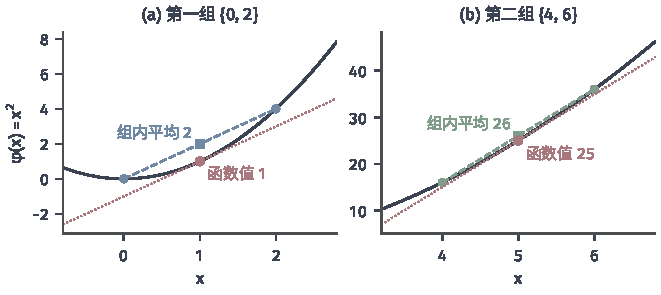
\includegraphics[width=112mm]{figures/02-abstract-mathematics/02-probability-spaces/matplotlib/cond-jensen/figure.pdf}
  \caption{条件Jensen不等式在四点空间两组上的表现，$\varphi(x)=x^2$。黑色曲线为$\varphi$，同色圆点为组内两点$(x,\varphi(x))$，虚线为连接它们的弦，方块为弦的中点即组内$\varphi$值的平均，红色圆点为条件平均处的函数值，红色点线为该处的支撑直线。(a)第一组$\{0,2\}$；(b)第二组$\{4,6\}$。}
  \label{fig:cond-jensen}
\end{figure}

\paragraph{矩收缩与平均误差的收缩}
取$\varphi(x)=|x|^p$（$p\geq1$）得到下面的推论，它说明条件平均不会放大矩，也不会放大两个变量之间的平均误差。

\begin{theorem}[推论：条件期望的收缩]
\label{thm:cond-contraction}
设$p\geq1$且$\mathbb E|X|^p<\infty$。则$|\mathbb E[X\mid\mathcal G]|^p\leq\mathbb E[|X|^p\mid\mathcal G]$几乎必然成立，从而
\[
  \mathbb E\bigl|\mathbb E[X\mid\mathcal G]\bigr|^p\leq\mathbb E|X|^p.
\]
特别地，对可积的$X,X'$，
\begin{equation}
  \mathbb E\bigl|\mathbb E[X\mid\mathcal G]-\mathbb E[X'\mid\mathcal G]\bigr|=\mathbb E\bigl|\mathbb E[X-X'\mid\mathcal G]\bigr|\leq\mathbb E|X-X'|.
  \label{eq:cond-l1-contraction}
\end{equation}
\end{theorem}

\begin{proof}
由$p\geq1$与$\mathbb E|X|^p<\infty$，第~\ref{chap:probability-models}章的矩单调性（定理~\ref{thm:pmod-moment-monotone}）给出$\mathbb E|X|<\infty$，于是$X$与$\varphi(X)=|X|^p$都可积。
$\varphi$是凸函数，由定理~\ref{thm:cond-jensen}得第一式；两边取期望并用全期望公式得第二式。
式~\eqref{eq:cond-l1-contraction}中的等号来自线性，不等号是$p=1$时对$X-X'$应用第二式。
\end{proof}

式~\eqref{eq:cond-l1-contraction}说，若$X_n$在平均绝对误差意义下接近$X$，那么在同一信息下取条件期望后仍然如此；第~\ref{chap:random-variable-convergence}章讨论平均收敛时会用到这个估计。

\paragraph{条件均方误差的分解}
现在把误差问题限定为：只依据$\mathcal G$中的信息给出一个预测$Z$，用均方误差$\mathbb E(X-Z)^2$衡量它离$X$多远。
候选预测是满足$\mathbb EZ^2<\infty$的$\mathcal G$可测随机变量，$X$也假设平方可积。
直观上，条件平均已经用尽了$\mathcal G$中的信息，其他预测与它的差距只会增加误差。

\begin{theorem}[条件均方误差最小]
\label{thm:cond-mse}
设$\mathbb EX^2<\infty$，$M=\mathbb E[X\mid\mathcal G]$。则$\mathbb EM^2\leq\mathbb EX^2$，并且对每个满足$\mathbb EZ^2<\infty$的$\mathcal G$可测随机变量$Z$，
\begin{equation}
  \mathbb E(X-Z)^2=\mathbb E(X-M)^2+\mathbb E(M-Z)^2.
  \label{eq:cond-mse-decomposition}
\end{equation}
因此$M$在这类预测中使均方误差最小，而且最小值只在$Z=M$几乎必然成立时达到。
\end{theorem}

\begin{proof}
$\mathbb EM^2\leq\mathbb EX^2$是定理~\ref{thm:cond-contraction}取$p=2$的情形。
把$X-Z$写成$(X-M)+(M-Z)$并展开平方，只需证明交叉项$\mathbb E[(X-M)(M-Z)]=0$。
令$H=M-Z$，它对$\mathcal G$可测且平方可积。由Cauchy--Schwarz不等式（定理~\ref{thm:pmod-cauchy-schwarz}），$HX$与$HM$都可积。
对$HX$用定理~\ref{thm:cond-pull-out}与全期望公式，
\[
  \mathbb E[HX]=\mathbb E\bigl[\mathbb E[HX\mid\mathcal G]\bigr]=\mathbb E[HM],
\]
即$\mathbb E[H(X-M)]=0$。于是式~\eqref{eq:cond-mse-decomposition}成立。
等式右边第二项非负，且为零当且仅当$Z=M$几乎必然成立，由此得到最小性与唯一性。
\end{proof}

式~\eqref{eq:cond-mse-decomposition}把任一预测的误差拆成两部分：$\mathbb E(X-M)^2$是只用$\mathcal G$时无论如何都消除不了的误差，$\mathbb E(M-Z)^2$是预测偏离条件平均的代价。
取平凡信息，$M=\mathbb EX$，分解就是熟悉的$\mathbb E(X-c)^2=\operatorname{Var}X+(\mathbb EX-c)^2$。
这里只用了展开平方和交叉项为零这一个恒等式；把条件期望看成函数空间中的正交投影，是第~\ref{part:function-spaces}部分的内容。

图~\ref{fig:cond-mse-decomposition}在示例~\ref{ex:cond-square-noise}的模型中（$\sigma^2=0.25$）比较四个只依赖$Y$的预测。
蓝色部分对四个预测都是$\mathbb E(X-M)^2=\mathbb E\varepsilon^2=0.25$；黄色部分是$\mathbb E(M-Z)^2$，常数预测$Z=1$为$\operatorname{Var}(Y^2)=2$，$Z=|Y|$为$\mathbb E(Y^2-|Y|)^2=4-4\sqrt{2/\pi}\approx0.808$，$Z=0.8Y^2$为$0.04\,\mathbb EY^4=0.12$。
菱形是用$400000$个模拟样本算出的均方误差，与两部分之和吻合。
蓝色底座的高度不随预测改变，这就是“无论怎样利用$Y$都消除不了的误差”。

\begin{figure}[htbp]
  \centering
  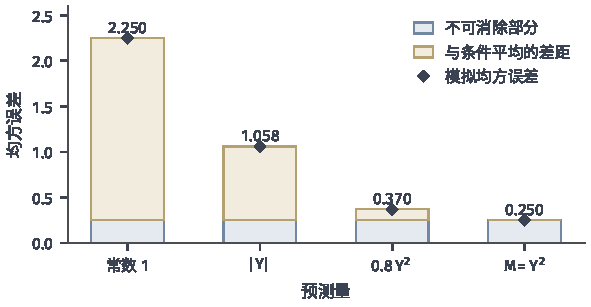
\includegraphics[width=100mm]{figures/02-abstract-mathematics/02-probability-spaces/matplotlib/cond-mse-decomposition/figure.pdf}
  \caption{条件均方误差分解~\eqref{eq:cond-mse-decomposition}的数值对照。模型为$Y\sim N(0,1)$，$\varepsilon\sim N(0,0.25)$与$Y$独立，$X=Y^2+\varepsilon$，$M=\mathbb E[X\mid Y]=Y^2$。每根柱子对应一个$\sigma(Y)$可测预测$Z$：蓝色为$\mathbb E(X-M)^2=0.25$，黄色为精确计算的$\mathbb E(M-Z)^2$，柱顶数字为二者之和；菱形为固定随机种子下$400000$个样本的经验均方误差。}
  \label{fig:cond-mse-decomposition}
\end{figure}

\subsection{固定信息下的条件极限}

\paragraph{取无穷值的条件期望}
交换条件期望与极限时，常常遇到不一定可积的非负随机变量，例如单调上升列的极限。
为此先把条件期望推广到非负随机变量，允许它取$+\infty$。

设$X\geq0$。截断$X\wedge n=\min(X,n)$有界，因而可积；由保序性，$Z_n=\mathbb E[X\wedge n\mid\mathcal G]$几乎必然单调不减；在单调性失效的那个零概率事件（它属于$\mathcal G$）上，把各$Z_n$都改为$0$，这只换了版本，此后可设$Z_n$处处单调不减。
定义
\[
  \mathbb E[X\mid\mathcal G]=\lim_{n\to\infty}\mathbb E[X\wedge n\mid\mathcal G],
\]
它是取值于$[0,\infty]$的$\mathcal G$可测随机变量。
对每个$A\in\mathcal G$，两边分别用单调收敛定理，
\[
  \mathbb E\bigl[\mathbb E[X\mid\mathcal G]\mathbb I_A\bigr]=\lim_n\mathbb E[Z_n\mathbb I_A]=\lim_n\mathbb E[(X\wedge n)\mathbb I_A]=\mathbb E[X\mathbb I_A],
\]
所以积分刻画~\eqref{eq:cond-defining-identity}照样成立，两边允许同为$+\infty$。

这一推广仍然几乎必然唯一。
若$Z,Z'$都是取值于$[0,\infty]$的$\mathcal G$可测随机变量，且对每个$A\in\mathcal G$满足$\mathbb E[Z\mathbb I_A]=\mathbb E[Z'\mathbb I_A]=\mathbb E[X\mathbb I_A]$，令$A_k=\{Z<Z',\,Z\leq k\}\in\mathcal G$。
则$\mathbb E[Z'\mathbb I_{A_k}]=\mathbb E[Z\mathbb I_{A_k}]\leq k$，所以$Z'$在$A_k$上几乎必然有限，$(Z'-Z)\mathbb I_{A_k}$非负且积分为零，得$\mathbb P(A_k)=0$。
对$k$取可数并得$\mathbb P(Z<Z')=0$，对称地得$\mathbb P(Z'<Z)=0$。
当$X$本身可积时，这一定义与定义~\ref{def:cond-expectation}一致。

\paragraph{条件单调收敛与条件Fatou}
有了非负情形的定义，普通积分中的单调收敛定理与Fatou引理都有固定信息下的版本。

\begin{theorem}[条件单调收敛定理与条件Fatou引理]
\label{thm:cond-monotone}
固定子$\sigma$代数$\mathcal G$。
\begin{enumerate}
  \item 若$0\leq X_n\uparrow X$几乎必然成立，则$\mathbb E[X_n\mid\mathcal G]\uparrow\mathbb E[X\mid\mathcal G]$几乎必然成立。
  \item 若$X_n\geq0$，则$\mathbb E[\liminf_nX_n\mid\mathcal G]\leq\liminf_n\mathbb E[X_n\mid\mathcal G]$几乎必然成立。
\end{enumerate}
其中的条件期望均按上一段取值于$[0,\infty]$。
\end{theorem}

\begin{proof}
(1) 对每个截断水平$k$，$X_n\wedge k\leq X_{n+1}\wedge k$，由保序性与极限定义，$Z_n=\mathbb E[X_n\mid\mathcal G]$几乎必然单调不减。令$Z=\lim_nZ_n$，它对$\mathcal G$可测。对每个$A\in\mathcal G$，两次使用单调收敛定理，
\[
  \mathbb E[Z\mathbb I_A]=\lim_n\mathbb E[Z_n\mathbb I_A]=\lim_n\mathbb E[X_n\mathbb I_A]=\mathbb E[X\mathbb I_A].
\]
由上一段的唯一性，$Z=\mathbb E[X\mid\mathcal G]$。

(2) 令$Y_n=\inf_{k\geq n}X_k$，则$0\leq Y_n\uparrow\liminf_kX_k$。对每个$k\geq n$，$Y_n\leq X_k$，由保序性$\mathbb E[Y_n\mid\mathcal G]\leq\mathbb E[X_k\mid\mathcal G]$；可数个$k$的例外零集合并后，得$\mathbb E[Y_n\mid\mathcal G]\leq\inf_{k\geq n}\mathbb E[X_k\mid\mathcal G]$。由(1)令$n\to\infty$，左边上升到$\mathbb E[\liminf_kX_k\mid\mathcal G]$，右边上升到$\liminf_k\mathbb E[X_k\mid\mathcal G]$。
\end{proof}

\paragraph{条件控制收敛}
最常用的是控制收敛的条件版本。
它的证明思路是把“误差趋于零”改写成一个单调上升列，再借助条件单调收敛；减法步骤需要控制变量的条件期望有限。

\begin{theorem}[条件控制收敛定理]
\label{thm:cond-dominated}
设$X_n\to X$几乎必然成立，并存在可积随机变量$Y$，使$|X_n|\leq Y$对每个$n$几乎必然成立。则
\[
  \mathbb E\bigl[|X_n-X|\bigm|\mathcal G\bigr]\to0,\qquad
  \mathbb E[X_n\mid\mathcal G]\to\mathbb E[X\mid\mathcal G]\qquad\text{几乎必然}.
\]
\end{theorem}

\begin{proof}
由$|X_n|\leq Y$与$X_n\to X$得$|X|\leq Y$，所以$X$可积。
令$U_n=\sup_{k\geq n}|X_k-X|$，则$U_n\downarrow0$且$0\leq U_n\leq2Y$几乎必然成立。
于是$0\leq2Y-U_n\uparrow2Y$，由定理~\ref{thm:cond-monotone}，
\[
  \mathbb E[2Y-U_n\mid\mathcal G]\uparrow\mathbb E[2Y\mid\mathcal G]\qquad\text{几乎必然}.
\]
$Y$与$U_n$都可积，$\mathbb E[Y\mid\mathcal G]$几乎必然有限，所以可以用线性把左边写成$2\mathbb E[Y\mid\mathcal G]-\mathbb E[U_n\mid\mathcal G]$，两边减去有限的$2\mathbb E[Y\mid\mathcal G]$，得$\mathbb E[U_n\mid\mathcal G]\downarrow0$。
由保序性，$\mathbb E[|X_n-X|\mid\mathcal G]\leq\mathbb E[U_n\mid\mathcal G]$，第一式得证；再由定理~\ref{thm:cond-rules}的绝对值规则，
\[
  \bigl|\mathbb E[X_n\mid\mathcal G]-\mathbb E[X\mid\mathcal G]\bigr|\leq\mathbb E\bigl[|X_n-X|\bigm|\mathcal G\bigr],
\]
第二式得证。
\end{proof}

证明中“减去有限的$2\mathbb E[Y\mid\mathcal G]$”一步说明了控制变量可积的作用：若条件期望可以取$+\infty$，就会出现$\infty-\infty$。
没有控制时结论可以失败。
取平凡信息，$\Omega=(0,1)$上$X_n=n\mathbb I_{(0,1/n)}$几乎处处趋于$0$，但$\mathbb E[X_n\mid\mathcal G]=\mathbb EX_n=1$不趋于$0$；第~\ref{chap:random-variable-convergence}章示例~\ref{ex:conv-spike}会从平均误差的角度重新分析这个例子。

本小节的所有陈述都固定同一个$\mathcal G$。
依概率收敛、一致可积与平均收敛之间的关系属于第~\ref{chap:random-variable-convergence}章；信息本身随时间增加时条件期望的极限，例如鞅收敛，属于\BookPartRef{part:dynamical-systems-control-decision-and-games}{卷三“过程与轨迹演化”部分}。

\section{概率核}
\label{sec:cond-kernels}

条件期望逐个处理可积变量；条件分布则要求对每个观测值同时给出一整个概率分布，并且这些分布随观测值可测地变化。
描述这种“输入一个状态，输出一个概率分布”的对象就是概率核。
本节先独立建立概率核、核积分、由核构造联合分布以及核的复合，下一节再用它准确表述条件分布。
这里只处理概率核：上一部分在测度层面讨论了推前与密度，概率核把确定的映射推广为随机的输出，所需的可测性与积分交换都在本节证明。

\subsection{概率核的定义}

\paragraph{有限集合上的随机矩阵}
先看有限的情形。
设输入状态集合$S=\{1,2,3\}$，输出状态集合$T=\{a,b,c\}$。
一张非负矩阵$K=(K(s,t))$，若每一行之和都是$1$，就称为随机矩阵；第$s$行是输入为$s$时输出的概率分布。
图~\ref{fig:cond-finite-kernel}给出一个例子：输入$2$以概率$0.2,0.6,0.2$分别输出$a,b,c$，三行之和都是$1$。
对输出集合$B\subseteq T$，记$K(s,B)=\sum_{t\in B}K(s,t)$，它是输入为$s$时输出落入$B$的概率。

\begin{figure}[htbp]
  \centering
  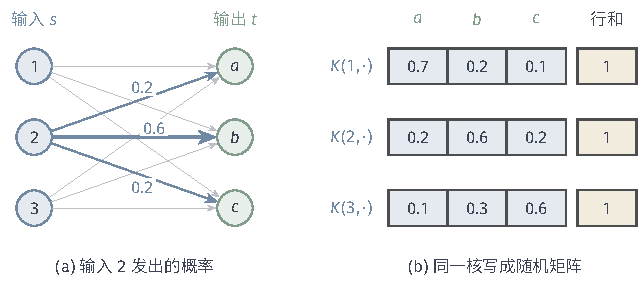
\includegraphics[width=108mm]{figures/02-abstract-mathematics/02-probability-spaces/tikz/cond-finite-kernel/figure.pdf}
  \caption{有限随机矩阵作为概率核。输入$S=\{1,2,3\}$，输出$T=\{a,b,c\}$。(a)以输入$2$为例，蓝色箭头上的数是它输出各状态的概率，灰线表示其余输入的转移；(b)同一核写成随机矩阵，第$s$行是分布$K(s,\cdot)$，右侧黄色格为行和$1$。}
  \label{fig:cond-finite-kernel}
\end{figure}

\paragraph{一般可测空间上的概率核}
在一般空间中，输入可以有不可数多个，输出的“行”也不再是有限向量。
随机矩阵的两项性质需要分别推广：固定输入时，输出端必须是一个概率测度；固定输出事件时，它的概率随输入的变化必须可测，否则无法再对输入求平均。

\begin{definition}[概率核]
\label{def:cond-kernel}
设$(S,\mathcal S)$与$(T,\mathcal T)$是可测空间。映射$K:S\times\mathcal T\to[0,1]$若满足
\begin{enumerate}
  \item 对每个$s\in S$，$K(s,\cdot)$是$(T,\mathcal T)$上的概率测度；
  \item 对每个$B\in\mathcal T$，$s\mapsto K(s,B)$是$\mathcal S$可测函数，
\end{enumerate}
则称$K$为从$S$到$T$的\term{概率核}（probability kernel）。
\end{definition}

它就是总质量为$1$的测度核。
第一项保证每个输入给出合法的输出分布，第二项保证当输入本身随机时，$\mathbb P(\text{输出}\in B)$可以通过对输入积分来计算。
有限情形中第二项自动成立，因为有限集合上（取全部子集为可测集时）的每个函数都可测。

\paragraph{确定性核与密度核}
两类常见的核位于两个极端。
设$f:S\to T$可测，令
\[
  K(s,B)=\mathbb I_B(f(s)),
\]
即输入$s$时以概率$1$输出$f(s)$。固定$s$时$K(s,\cdot)$是单点质量；固定$B$时$s\mapsto\mathbb I_B(f(s))=\mathbb I_{f^{-1}(B)}(s)$可测，正是因为$f$可测。
这称为\term{确定性核}（deterministic kernel），可测映射因此可以看成没有随机性的核。

另一端是密度核。
设$\lambda$是$(T,\mathcal T)$上的$\sigma$有限测度，$k:S\times T\to[0,\infty)$对$\mathcal S\otimes\mathcal T$可测，并且对每个$s$有$\int_Tk(s,t)\,\lambda(dt)=1$。令
\[
  K(s,B)=\int_Bk(s,t)\,\lambda(dt).
\]
固定$s$时，这是密度为$k(s,\cdot)$的概率测度；固定$B$时，$s\mapsto K(s,B)$的可测性来自一般的Tonelli定理（第~\ref{sec:integral-tonelli}节），这也是要求$k$关于输入与输出\emph{联合}可测的原因。

图~\ref{fig:cond-kernel-types}把两类核的“行”画在一起，取$f(s)=s$。
左图中每个输入$s$只在$t=s$处放一个点质量；右图中每个输入给出以$s$为中心、标准差$0.15$的正态密度。
密度核的所有行都关于同一个Lebesgue测度有密度；确定性核的各行却没有共同的$\sigma$有限参考测度。
事实上，若$\sigma$有限测度$\lambda$使每个单点质量$\delta_s$（$s\in\mathbb R$）都关于$\lambda$绝对连续，则每个$\lambda(\{s\})>0$；但$\sigma$有限测度至多有可数个正质量的单点（每个有限质量的块中，质量超过$1/m$的单点至多有限个），矛盾。
所以概率核比“条件密度”适用得更广：没有共同参考密度时，核仍然存在。

\begin{figure}[htbp]
  \centering
  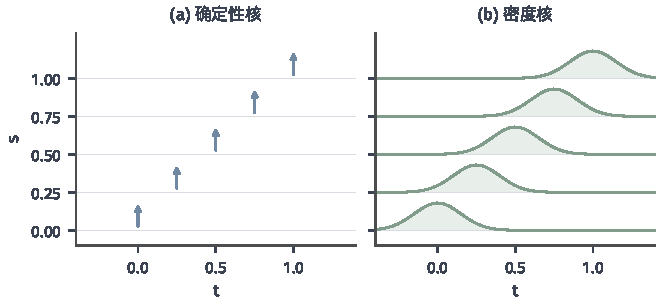
\includegraphics[width=112mm]{figures/02-abstract-mathematics/02-probability-spaces/matplotlib/cond-kernel-types/figure.pdf}
  \caption{两类概率核的行$K(s,\cdot)$，横轴为输出$t$，每条水平基线对应一个输入$s\in\{0,0.25,0.5,0.75,1\}$。(a)确定性核$K(s,\cdot)=\delta_{f(s)}$，$f(s)=s$，箭头表示单点质量；(b)密度核，$K(s,dt)$为$N(s,0.15^2)$，为便于比较，各密度曲线缩放到相同峰高。}
  \label{fig:cond-kernel-types}
\end{figure}

\subsection{核积分与联合分布}

\paragraph{核积分}
给定输入$s$后，对输出的函数$f$求平均，得到
\begin{equation}
  Kf(s)=\int_Tf(t)\,K(s,dt),
  \label{eq:cond-kernel-integral}
\end{equation}
这里$f$是非负可测函数（允许$Kf$取$+\infty$）或有界可测函数。
在有限情形，$Kf$就是随机矩阵乘以列向量$f$。

$Kf$作为输入的函数是可测的，证明沿积分的标准构造逐步进行。
若$f=\mathbb I_B$，则$Kf(s)=K(s,B)$，由核的第二项条件可测；对非负简单函数，$Kf$是可测函数的线性组合。
对非负可测$f$，取非负简单函数$f_n\uparrow f$，对每个固定的$s$用单调收敛定理得$Kf_n(s)\uparrow Kf(s)$，可测函数列的逐点极限仍可测。
对有界$f$，分别处理$f^+$与$f^-$，两者的核积分都有限。

\paragraph{输出分布}
若输入本身随机，服从$(S,\mathcal S)$上的概率分布$\mu$，那么输出落入$B$的总概率应当是各输入下概率的加权平均：
\[
  \mu K(B)=\int_SK(s,B)\,\mu(ds),\qquad B\in\mathcal T.
\]
由核的第二项条件，右边的被积函数可测。$\mu K(T)=1$；若$B_1,B_2,\ldots$两两不交，则$K(s,\bigcup_kB_k)=\sum_kK(s,B_k)$，对非负部分和用单调收敛定理得可数可加性。
所以$\mu K$是$(T,\mathcal T)$上的概率测度，称为输出分布。
同样从示性函数出发逐步推广，可得$\int_Tf\,d(\mu K)=\int_SKf\,d\mu$对非负或有界可测$f$成立。

在有限情形，$\mu K$就是行向量$\mu$乘随机矩阵$K$。
取$\mu=(0.5,0.3,0.2)$，图~\ref{fig:cond-finite-kernel}的核给出
\[
  \begin{aligned}
  \mu K&=0.5\,(0.7,0.2,0.1)+0.3\,(0.2,0.6,0.2)+0.2\,(0.1,0.3,0.6)\\
  &=(0.43,0.34,0.23).
  \end{aligned}
\]
输入的不确定性就这样按行加权传到输出。

\paragraph{由输入分布与核构造联合分布}
输出分布只记录了输出，丢掉了输入与输出的配对。
有限情形中，配对$(s,t)$的概率是$\mu(s)K(s,t)$，把它排成一张表，按列求和得到$\mu K$，按行求和得到$\mu$，如图~\ref{fig:cond-joint-from-kernel}所示。
一般情形下，我们希望对乘积空间中的集合$A$令
\[
  M(A)=\int_SK(s,A_s)\,\mu(ds),\qquad A_s=\{t\in T:(s,t)\in A\},
\]
即先固定输入$s$，用$K(s,\cdot)$度量$A$在$s$处的截面，再对$s$平均。
这需要先确认截面可测，并且$s\mapsto K(s,A_s)$可测。

\begin{figure}[htbp]
  \centering
  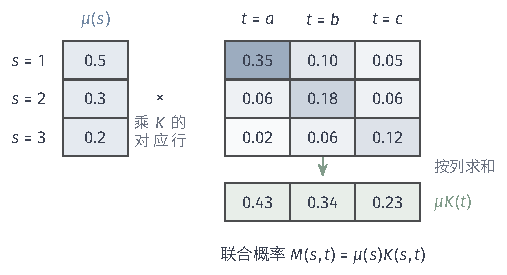
\includegraphics[width=86mm]{figures/02-abstract-mathematics/02-probability-spaces/tikz/cond-joint-from-kernel/figure.pdf}
  \caption{由输入分布与核构造联合分布。输入分布$\mu=(0.5,0.3,0.2)$，核$K$同图~\ref{fig:cond-finite-kernel}；中间表格的第$s$行是$\mu(s)$乘$K$的第$s$行，底色深浅与概率成正比；按列求和得到输出分布$\mu K=(0.43,0.34,0.23)$，按行求和则回到$\mu$。}
  \label{fig:cond-joint-from-kernel}
\end{figure}

\begin{theorem}[由输入分布与核构造联合分布]
\label{thm:cond-kernel-joint}
设$\mu$是$(S,\mathcal S)$上的概率测度，$K$是从$S$到$T$的概率核。则：
\begin{enumerate}
  \item 对每个$A\in\mathcal S\otimes\mathcal T$，截面$A_s\in\mathcal T$，且$s\mapsto K(s,A_s)$对$\mathcal S$可测；
  \item $M(A)=\int_SK(s,A_s)\,\mu(ds)$是$\mathcal S\otimes\mathcal T$上的概率测度，它是满足$M(B\times C)=\int_BK(s,C)\,\mu(ds)$（$B\in\mathcal S$，$C\in\mathcal T$）的唯一概率测度；
  \item 对非负的$\mathcal S\otimes\mathcal T$可测函数$f$，$s\mapsto\int_Tf(s,t)\,K(s,dt)$对$\mathcal S$可测，并且
  \begin{equation}
    \int_{S\times T}f\,dM=\int_S\Bigl(\int_Tf(s,t)\,K(s,dt)\Bigr)\mu(ds);
    \label{eq:cond-kernel-iterated}
  \end{equation}
  若$f$有符号且$\int|f|\,dM<\infty$，内层积分对$\mu$几乎每个$s$有限，式~\eqref{eq:cond-kernel-iterated}仍然成立。
\end{enumerate}
$M$的第一边缘是$\mu$，第二边缘是$\mu K$。
\end{theorem}

\begin{proof}
(1) 令$\mathcal D$为满足以下条件的$A\in\mathcal S\otimes\mathcal T$组成的族：每个截面$A_s\in\mathcal T$，且$s\mapsto K(s,A_s)$可测。
对可测矩形$B\times C$，截面在$s\in B$时为$C$，否则为空集，所以$K(s,(B\times C)_s)=\mathbb I_B(s)K(s,C)$可测，矩形属于$\mathcal D$。
若$A\in\mathcal D$，则$(A^c)_s=(A_s)^c$，$K(s,(A^c)_s)=1-K(s,A_s)$可测；若$A_1,A_2,\ldots\in\mathcal D$两两不交，则各截面两两不交，$K(s,(\bigcup_kA_k)_s)=\sum_kK(s,(A_k)_s)$是可测函数的级数和。
所以$\mathcal D$对补集与不交可数并封闭。可测矩形构成包含$S\times T$的$\pi$系统并生成$\mathcal S\otimes\mathcal T$，由$\pi$--$\lambda$定理，$\mathcal D=\mathcal S\otimes\mathcal T$。

(2) 由(1)，$M$有定义，且$M(S\times T)=1$。若$A_k$两两不交，对$K(s,(\bigcup_kA_k)_s)=\sum_kK(s,(A_k)_s)$用单调收敛定理得$M(\bigcup_kA_k)=\sum_kM(A_k)$。矩形公式就是(1)中的计算。两个在矩形上取值相同的概率测度，由定理~\ref{thm:measure-uniqueness}在整个乘积$\sigma$代数上相等。

(3) 对$f=\mathbb I_A$，内层积分为$K(s,A_s)$，式~\eqref{eq:cond-kernel-iterated}就是$M$的定义。由线性推广到非负简单函数；对一般非负$f$，取非负简单函数$f_n\uparrow f$，内层对每个$s$用单调收敛定理，外层再用一次，可测性与等式都保留。
对绝对可积的$f$，对$|f|$用非负情形知内层积分$\int|f(s,t)|K(s,dt)$对$\mu$几乎每个$s$有限；在这些$s$上把$f=f^+-f^-$的两部分分别代入并相减即可。

取$A=B\times T$与$A=S\times C$，分别得$M(B\times T)=\mu(B)$与$M(S\times C)=\mu K(C)$。
\end{proof}

我们把这个联合分布记作$\mu(ds)K(s,dt)$，或简记为$\mu\otimes K$。
当$K(s,\cdot)=\nu$不依赖$s$时，它就是乘积测度$\mu\otimes\nu$，联合分布中输入与输出独立；一般的核则让输出分布随输入改变，从而在联合分布中建立依赖。
本节从输入分布和核出发得到联合分布；下一节研究反方向的问题：给定联合分布，怎样恢复以一个坐标为输入的条件核。

\subsection{概率核的复合}

\paragraph{先平均中间状态}
设$K$是从$S$到$T$的概率核，$L$是从$T$到$U$的概率核。
输入$s$先经$K$得到中间状态$t$，再经$L$得到输出$u$；我们只关心从$s$到$u$的规律，因此对中间状态求平均：
\[
  (KL)(s,C)=\int_TL(t,C)\,K(s,dt),\qquad s\in S,\ C\in\mathcal U.
\]
用核积分的记号，$(KL)(s,C)=K\bigl(L(\cdot,C)\bigr)(s)$。

\begin{lemma}[核的复合与结合律]
\label{lem:cond-kernel-composition}
$KL$是从$S$到$U$的概率核，并且对非负可测$g$有$(KL)g=K(Lg)$。若再给定从$U$到$V$的概率核$N$，则$(KL)N=K(LN)$。
\end{lemma}

\begin{proof}
固定$C$，$t\mapsto L(t,C)$是取值于$[0,1]$的可测函数，由核积分的可测性，$s\mapsto(KL)(s,C)$可测。
固定$s$，$(KL)(s,U)=1$；若$C_k$两两不交，$L(t,\bigcup_kC_k)=\sum_kL(t,C_k)$，对$K(s,dt)$积分并用单调收敛定理得可数可加性。所以$KL$是概率核。
等式$(KL)g=K(Lg)$对$g=\mathbb I_C$就是定义；由线性推广到非负简单函数，再在两边逐层用单调收敛定理推广到非负可测$g$。
最后，对$D\in\mathcal V$，令$g=N(\cdot,D)$，则$((KL)N)(s,D)=(KL)g(s)=K(Lg)(s)=(K(LN))(s,D)$。
\end{proof}

在有限集合上，$(KL)(s,u)=\sum_tK(s,t)L(t,u)$，复合就是随机矩阵的乘法，结合律就是矩阵乘法的结合律。
同样可以验证$\mu(KL)=(\mu K)L$：先把输入分布推到中间，再推到输出，与直接用复合核推送结果相同。

\paragraph{两个翻转核}
取$S=T=U=\{0,1\}$。
第一个核以概率$p$翻转比特、以概率$1-p$保持不变，第二个核的翻转概率为$q$。
从输入$0$到输出$1$有两条路径：先保持再翻转，概率$(1-p)q$；先翻转再保持，概率$p(1-q)$。
对中间状态求和，复合核的翻转概率为
\[
  (KL)(0,\{1\})=p(1-q)+(1-p)q.
\]
取$p=0.1$，$q=0.2$，得$0.08+0.18=0.26$，如图~\ref{fig:cond-kernel-composition}所示。
复合后仍是一个翻转核，并且满足$1-2\times0.26=0.48=(1-2p)(1-2q)$：用$\pm1$编码比特时，$1-2p$是输出与输入乘积的平均，经过两次翻转，这一乘积平均相乘。

\begin{figure*}[htbp]
  \centering
  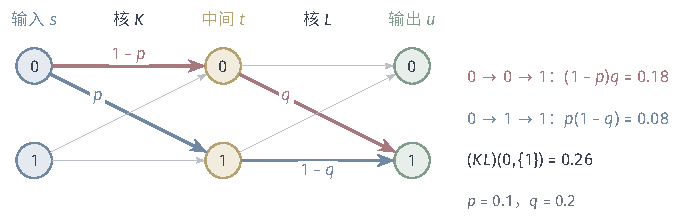
\includegraphics[width=115mm]{figures/02-abstract-mathematics/02-probability-spaces/tikz/cond-kernel-composition/figure.pdf}
  \caption{两个二元翻转核的复合。核$K$的翻转概率为$p=0.1$，核$L$的翻转概率为$q=0.2$。从输入$0$到输出$1$的两条路径分别用红色（$0\to0\to1$）与蓝色（$0\to1\to1$）标出，灰线为其余转移；两条路径的概率相加得到复合核的翻转概率$0.26$。}
  \label{fig:cond-kernel-composition}
\end{figure*}

本节只处理有限个核的复合以及由一个核构造联合分布。
沿时间不断复合核得到的过程模型、Markov性，以及无限序列上联合分布的存在性，与上一节提到的鞅收敛一样，都留给卷三的过程部分。

\section{条件分布}
\label{sec:cond-distributions}

有了概率核的语言，我们可以把逐个事件的条件概率组织成一个整体对象。
本节依次回答四个问题：这个对象怎样定义，何时存在、在什么意义下唯一，怎样用它计算条件平均，以及有密度时怎样具体写出它。

\subsection{条件分布的定义}

\paragraph{从逐事件条件概率到一个核}
设$X$是取值于可测空间$(E,\mathcal E)$的随机对象，$\mathcal G\subseteq\mathcal F$是子$\sigma$代数。
对每个$B\in\mathcal E$，第~\ref{sec:cond-definition}节给出条件概率$\mathbb P(X\in B\mid\mathcal G)$，但它只是一个几乎必然确定的版本。
我们希望一次选好所有版本，使它们在每个样本点处共同构成$E$上的一个概率分布。

\begin{definition}[正则条件分布]
\label{def:cond-regular-distribution}
设$X$取值于$(E,\mathcal E)$，$\mathcal G\subseteq\mathcal F$是子$\sigma$代数。
若$K_{\mathcal G}$是从$(\Omega,\mathcal G)$到$(E,\mathcal E)$的概率核，并且对每个$B\in\mathcal E$，
\[
  K_{\mathcal G}(\cdot,B)=\mathbb P(X\in B\mid\mathcal G)\qquad\text{几乎必然},
\]
即$K_{\mathcal G}(\cdot,B)$是条件概率$\mathbb P(X\in B\mid\mathcal G)$的一个版本，则称$K_{\mathcal G}$为$X$给定$\mathcal G$的\term{正则条件分布}（regular conditional distribution）。
\end{definition}

定义包含两项不同的要求。
第一项是逐事件的：每个$K_{\mathcal G}(\cdot,B)$都对$\mathcal G$可测，并在$\mathcal G$的事件上保持概率。
第二项是整体的：对每个固定的$\omega$，$B\mapsto K_{\mathcal G}(\omega,B)$必须是概率测度。
逐事件的条件概率总是存在，但每个版本都可以在各自的零概率事件上任意改动；第二项要求所有这些改动在同一个$\omega$处相容，这并不自动成立。

\paragraph{以观测值为输入的条件核}
信息由观测$Y$给出时，我们更希望条件分布直接以观测值为输入。
设$Y$取值于$(D,\mathcal D)$。若$K$是从$D$到$E$的概率核，且对每个$B\in\mathcal E$，
\[
  K(Y,B)=\mathbb P(X\in B\mid Y)\qquad\text{几乎必然},
\]
就称$K$为$X$给定$Y$的条件分布（或条件核），并记
\[
  \mathbb P(X\in B\mid Y=y)=K(y,B).
\]
此时$\omega\mapsto K(Y(\omega),\cdot)$是$X$给定$\sigma(Y)$的正则条件分布：它对$\sigma(Y)$可测，因为$K(\cdot,B)$可测而$Y$可测。

由式~\eqref{eq:cond-given-y-identity}，上述要求等价于对每个$B\in\mathcal E$、$C\in\mathcal D$，
\begin{equation}
  \mathbb P(X\in B,\,Y\in C)=\int_CK(y,B)\,P_Y(dy).
  \label{eq:cond-kernel-disintegration}
\end{equation}
对照定理~\ref{thm:cond-kernel-joint}，这说明$(Y,X)$的联合分布正是$P_Y(dy)K(y,dx)$：两者在可测矩形上一致，由唯一性在整个乘积$\sigma$代数上一致。
所以条件核就是把联合分布按第一个坐标分解所得的核，即联合分布的一种核分解。

记号$\mathbb P(X\in B\mid Y=y)$来自条件核，而不是在$\mathbb P(Y=y)=0$时继续使用事件概率之比。
式~\eqref{eq:cond-kernel-disintegration}只对$y$积分，所以核在一个$P_Y$零集上的取值不受约束；条件核首先确定的是$P_Y$几乎处处意义下的条件规律。
例如$X=Y+\varepsilon$，其中$\varepsilon\sim N(0,1)$与$Y$独立，则$K(y,\cdot)=N(y,1)$满足式~\eqref{eq:cond-kernel-disintegration}，每个$\{Y=y\}$的概率是否为零都不影响这一说法。

\subsection{条件分布的存在性与版本}

\paragraph{实值情形：先在有理点上选版本}
为什么逐事件的条件概率不足以拼成分布？
$\mathcal E$中的事件通常有不可数多个，每个版本各带一个例外零集，不可数个零集的并可能不是零集，甚至不可测。
实值情形的出路是：分布由分布函数决定，而分布函数又由它在有理点上的值决定，于是只需在可数个点上选版本。

设$X$是实值随机变量。对每个有理数$r$，取$\mathbb P(X\leq r\mid\mathcal G)$的一个版本$G_r$。
下列三类性质对每个固定的有理数（或有理数对）几乎必然成立：
\begin{enumerate}
  \item 单调：$r<r'$时$G_r\leq G_{r'}$，由保序性得到；
  \item 有理点右连续：$G_{r+1/n}\to G_r$，因为$\mathbb I_{\{X\leq r+1/n\}}\downarrow\mathbb I_{\{X\leq r\}}$，由条件控制收敛定理~\ref{thm:cond-dominated}得到；
  \item 端点极限：整数$k\to-\infty$时$G_k\to0$，$k\to+\infty$时$G_k\to1$，同样由条件控制收敛得到。
\end{enumerate}
这些性质只涉及可数个有理数（或有理数对），各自的例外零集合并后，得到一个零概率事件$N\in\mathcal G$。

在$N$之外令
\[
  F(x,\omega)=\inf_{r\in\mathbb Q,\,r>x}G_r(\omega),\qquad x\in\mathbb R.
\]
它关于$x$单调不减、右连续，在$-\infty$与$+\infty$处的极限分别为$0$与$1$，因而是一个分布函数，唯一确定$\mathbb R$上的一个Borel概率测度$K_{\mathcal G}(\omega,\cdot)$。
在$N$上，令$K_{\mathcal G}(\omega,\cdot)$等于一个固定的概率测度，例如$N(0,1)$。
由有理点右连续与单调性，在$N$外$F(r,\omega)=G_r(\omega)$对每个有理数$r$成立。$G_r$只在有理点上选定，取$\inf_{r>x}$既把它延拓到全部实数，又保证延拓结果处处右连续，同时不改变有理点上已选好的值。

图~\ref{fig:cond-cdf-rationals}用一个有原子的例子展示这一构造。
设给定$Y=y$时$Z\sim N(y-0.5,0.25)$，$X=\max(Z,0)$，于是条件分布函数在$x<0$时为$0$，在$x\geq0$时为$\Phi\bigl((x-y+0.5)/0.5\bigr)$，在$0$处有跳跃。
左图中圆点是二进有理点上的值，曲线是由这些值右连续化得到的分布函数；右图取$y=0.5$，有理点$r=\frac12,\frac14,\frac18,\ldots$从右侧逼近$0$，函数值依次为$0.841,0.691,0.599,\ldots$，下确界$0.5$正是跳跃后的值$F(0\mid y)$。

\begin{figure}[htbp]
  \centering
  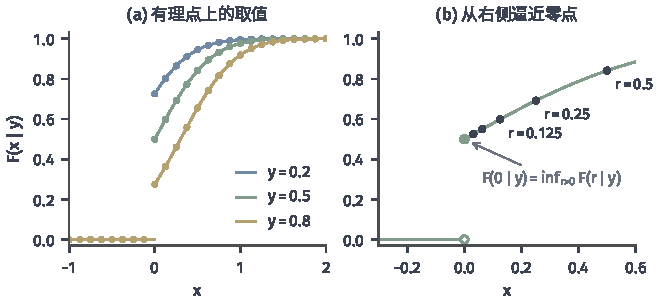
\includegraphics[width=112mm]{figures/02-abstract-mathematics/02-probability-spaces/matplotlib/cond-cdf-rationals/figure.pdf}
  \caption{由有理点上的值构造条件分布函数。模型为$X=\max(Z,0)$，给定$Y=y$时$Z\sim N(y-0.5,0.5^2)$，条件分布函数在$x=0$处跳跃$\Phi(1-2y)$。(a)$y=0.2,0.5,0.8$时，圆点为$x=k/8$（$k=-8,\ldots,16$）处的取值，曲线为右连续化后的分布函数；(b)$y=0.5$时，黑点为$r=2^{-1},\ldots,2^{-5}$处的取值，实心圆为$F(0\mid y)=0.5$，空心圆表示左极限$0$。}
  \label{fig:cond-cdf-rationals}
\end{figure}

\paragraph{标准Borel空间上的存在定理}
上面的构造用到了实数的两项结构：有理数是可数的稠密集，分布由分布函数决定。
对一般取值空间，相应的充分条件是\term{标准Borel空间}（standard Borel space）：与某个完备可分度量空间的Borel子集可测同构的可测空间。
实数、有限维欧氏空间及其Borel子集、可数离散空间都属于此类。

\begin{theorem}[正则条件分布的存在性]
\label{thm:cond-regular-existence}
\begin{enumerate}
  \item 设$X$是实值随机变量，或更一般地取值于标准Borel空间$(E,\mathcal E)$，$\mathcal G\subseteq\mathcal F$是任意子$\sigma$代数，则$X$给定$\mathcal G$的正则条件分布存在。
  \item 设$X$取值于标准Borel空间$(E,\mathcal E)$，$Y$取值于可测空间$(D,\mathcal D)$，则存在从$D$到$E$的概率核$K$，使$K(Y,B)=\mathbb P(X\in B\mid Y)$对每个$B\in\mathcal E$几乎必然成立。特别地，$X,Y$都取值于标准Borel空间时结论成立。
\end{enumerate}
\end{theorem}

\begin{proof}
\emph{实值情形的(1)。}沿用上一段的构造。$K_{\mathcal G}(\omega,\cdot)$对每个$\omega$是概率测度。对实数$x$，取有理数$r_k\downarrow x$，在$N$外$K_{\mathcal G}(\cdot,(-\infty,x])=\lim_kG_{r_k}$对$\mathcal G$可测；又$\mathbb I_{\{X\leq r_k\}}\downarrow\mathbb I_{\{X\leq x\}}$，由条件控制收敛，这个极限是$\mathbb P(X\leq x\mid\mathcal G)$的版本。
令$\mathcal D$为使$K_{\mathcal G}(\cdot,B)$对$\mathcal G$可测并且是$\mathbb P(X\in B\mid\mathcal G)$版本的Borel集$B$组成的族。它包含$\pi$系统$\{(-\infty,x]:x\in\mathbb R\}\cup\{\mathbb R\}$；对补集封闭，因为两边都是$1$减去原来的值；对不交可数并封闭，因为左边按测度可加，右边由条件单调收敛定理~\ref{thm:cond-monotone}可加。由$\pi$--$\lambda$定理，$\mathcal D$包含全部Borel集。

\emph{(2)的实值情形。}把上述构造中的$G_r$换成观测值上的函数：由定理~\ref{thm:cond-doob-dynkin}，$\mathbb P(X\leq r\mid Y)=g_r(Y)$，$g_r$在$D$上可测。三类性质的例外集写成$\{Y\in N'\}$，其中$N'\in\mathcal D$由$g_r$的可数个不等式与极限关系确定，而$P_Y(N')=\mathbb P(Y\in N')=0$。在$N'$外用$g_r(y)$构造分布函数，在$N'$上取固定分布，就得到以$y$为输入的核，其余验证与上一步相同。

\emph{标准Borel值的情形（证明思路，补充）。}标准Borel空间的分类定理（Kuratowski定理）表明，存在可测同构$\phi$把$E$映成$\mathbb R$的一个Borel子集$\phi(E)$。对实值随机变量$\phi(X)$得到条件核$\widetilde K$；由于$\mathbb P(\phi(X)\in\phi(E))=1$，$\widetilde K(\cdot,\phi(E))=1$在一个零集外成立，在该零集上把核改为$\phi(E)$上的固定分布，再用$\phi^{-1}$推回$E$即可。分类定理的证明属于描述集合论，这里只陈述而不展开。
\end{proof}

主线需要记住的是条件：逐个事件的条件概率在任意子$\sigma$代数下都存在，而要把它们拼成一个分布，本书使用“取值空间为标准Borel空间”这一充分条件。
这一条件约束的是$X$的取值空间；给定的信息$\mathcal G$或观测空间$D$不需要额外结构。

\paragraph{两个条件核在同一零集外一致}
条件核在什么意义下唯一？
设$K,K'$都是$X$给定$Y$的条件核，$E$是标准Borel空间。
标准Borel空间的$\sigma$代数可以由一个可数的$\pi$系统$\mathcal C$生成，不妨设$E\in\mathcal C$；例如$E=\mathbb R$时，取全部有理端点的半直线$(-\infty,r]$再添上$\mathbb R$。
对每个$C\in\mathcal C$，$K(Y,C)$与$K'(Y,C)$都是$\mathbb P(X\in C\mid Y)$的版本，因而$N_C=\{y:K(y,C)\neq K'(y,C)\}$是$P_Y$零集。
令$N=\bigcup_{C\in\mathcal C}N_C$，它仍是$P_Y$零集。对$y\notin N$，两个概率测度$K(y,\cdot)$与$K'(y,\cdot)$在$\pi$系统$\mathcal C$上一致，由定理~\ref{thm:measure-uniqueness}，它们在整个$\mathcal E$上相等。

所以两个条件核在一个\emph{共同的}$P_Y$零集之外，对全部目标事件同时相等。
这一结论比较的是两个已经是核的对象。
它并不表示事先为每个事件任意选取的条件概率版本都会与某个核在同一个零集外吻合：每个版本各自只在自己的零集外与核相等，不可数个这样的零集无法合并。

\subsection{条件分布的积分表示}

\paragraph{用一个核计算各种条件平均}
条件分布的价值在于：一旦给出整个核，所有可积函数的条件平均都可以由它统一计算，不必为每个函数另外寻找一个条件期望版本。

\begin{theorem}[条件分布的积分表示]
\label{thm:cond-kernel-integral}
设$K$是$X$给定$Y$的条件核，$X$取值于$(E,\mathcal E)$，$Y$取值于$(D,\mathcal D)$。
设$h:E\times D\to\mathbb R$对$\mathcal E\otimes\mathcal D$可测，并且非负或满足$\mathbb E|h(X,Y)|<\infty$。则$y\mapsto\int_Eh(x,y)\,K(y,dx)$可测（可积情形下在一个$P_Y$零集外有定义），并且
\begin{equation}
  \mathbb E[h(X,Y)\mid Y]=\int_Eh(x,Y)\,K(Y,dx)\qquad\text{几乎必然}.
  \label{eq:cond-kernel-integral-representation}
\end{equation}
特别地，对非负或满足$\mathbb E|f(X)|<\infty$的可测$f:E\to\mathbb R$，$\mathbb E[f(X)\mid Y]=\int_Ef(x)\,K(Y,dx)$；两边再取期望得
\[
  \mathbb E\,h(X,Y)=\int_D\Bigl(\int_Eh(x,y)\,K(y,dx)\Bigr)P_Y(dy).
\]
\end{theorem}

\begin{proof}
内层积分的可测性来自定理~\ref{thm:cond-kernel-joint}（输入为$y$，输出为$x$）。
先设$h=\mathbb I_{B\times C}$，$B\in\mathcal E$，$C\in\mathcal D$。右边是$\mathbb I_C(Y)K(Y,B)=\mathbb I_C(Y)\,\mathbb P(X\in B\mid Y)$；由提出已知因子（定理~\ref{thm:cond-pull-out}），它等于$\mathbb E[\mathbb I_C(Y)\mathbb I_B(X)\mid Y]$。
令$\mathcal A$为使式~\eqref{eq:cond-kernel-integral-representation}对$h=\mathbb I_A$成立的$A\in\mathcal E\otimes\mathcal D$组成的族。它包含可测矩形；对补集封闭，因为两边对$\mathbb I_{E\times D}=1$都成立并且线性；对不交可数并封闭，因为左边由条件单调收敛定理可加，右边由单调收敛定理可加。由$\pi$--$\lambda$定理，$\mathcal A=\mathcal E\otimes\mathcal D$。
由线性推广到非负简单函数；对非负$h$，取非负简单函数$h_n\uparrow h$，左边用条件单调收敛，右边对每个$y$用单调收敛。
对$\mathbb E|h(X,Y)|<\infty$的情形，非负结论与全期望公式给出$\mathbb E\int|h(x,Y)|K(Y,dx)=\mathbb E|h(X,Y)|<\infty$，所以内层积分在一个$P_Y$零集外有限；分别对$h^+,h^-$使用非负结论再相减。
最后一式是对式~\eqref{eq:cond-kernel-integral-representation}取期望，并用换元公式把对$Y$的期望写成对$P_Y$的积分。
\end{proof}

给定$Y=y$后为什么只对$x$积分？因为$y$已经被观察到，$h(\cdot,y)$中的第二个坐标是已知常数，剩下的不确定性只来自$X$，而它的规律由$K(y,\cdot)$描述。
这正是提出已知因子的“分布版本”。

\paragraph{先条件、后平均：有限混合}
最后一式把一个联合期望拆成两步：先在每个观测值下按条件分布求平均，再按观测值的分布平均。
这是定理~\ref{thm:cond-kernel-joint}正向构造的逆读：那里由$P_Y$与$K$拼出联合分布，这里把联合期望按同样的结构拆开。

\begin{example}[两分量正态混合]
\label{ex:cond-mixture}
设类别$Y$取值$1,2$，$\mathbb P(Y=1)=0.4$，$\mathbb P(Y=2)=0.6$；给定$Y=1$时$X\sim N(0,1)$，给定$Y=2$时$X\sim N(3,1)$。
条件核为$K(1,\cdot)=N(0,1)$、$K(2,\cdot)=N(3,1)$，$X$的分布是混合$0.4\,N(0,1)+0.6\,N(3,1)$。
取同时依赖两个坐标的$h(x,y)=\mathbb I_{\{x>y\}}$，先条件：
\[
  \begin{aligned}
  \mathbb P(X>Y\mid Y=1)&=\mathbb P(N(0,1)>1)\approx0.159,\\
  \mathbb P(X>Y\mid Y=2)&=\mathbb P(N(3,1)>2)\approx0.841,
  \end{aligned}
\]
再平均：$\mathbb P(X>Y)\approx0.4\times0.159+0.6\times0.841\approx0.568$。
用固定随机种子模拟$200000$次，得到的频率约为$0.569$。
同样，$\mathbb E[X^2\mid Y]$在$Y=1,2$时分别为$1$与$3^2+1=10$，于是$\mathbb EX^2=0.4\times1+0.6\times10=6.4$。
\end{example}

图~\ref{fig:cond-mixture-two-stage}左图把两个条件密度按类别概率加权，阴影部分分别是$x>1$与$x>2$的区域，虚线是两者之和即混合密度；右图是每个类别下的条件概率，红色虚线是按类别概率加权后的平均。
只看$X$的混合密度无法算出$\mathbb P(X>Y)$：阈值随类别变化，而混合密度已经把类别信息平均掉了。先条件、后平均把问题拆成了两个普通的正态尾概率。

\begin{figure}[htbp]
  \centering
  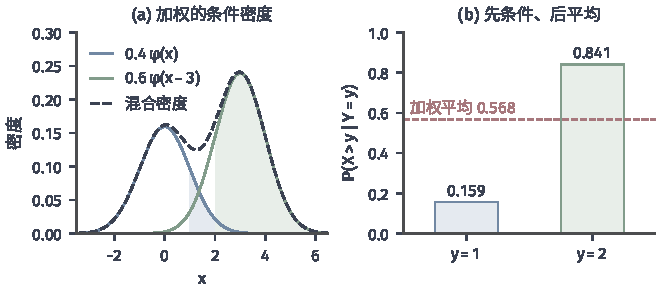
\includegraphics[width=112mm]{figures/02-abstract-mathematics/02-probability-spaces/matplotlib/cond-mixture-two-stage/figure.pdf}
  \caption{有限混合分布中“先条件、后平均”的计算。$\mathbb P(Y=1)=0.4$，$\mathbb P(Y=2)=0.6$，给定$Y=1,2$时$X$分别服从$N(0,1)$与$N(3,1)$，$\varphi$为标准正态密度。(a)加权条件密度与混合密度（虚线），阴影为$x>y$的区域；(b)两类别下的条件概率$\mathbb P(X>y\mid Y=y)$及其加权平均$0.568$（红色虚线）。}
  \label{fig:cond-mixture-two-stage}
\end{figure}

\subsection{条件密度与Bayes公式}

\paragraph{由联合密度构造条件核}
具体计算条件核时，最常见的情形是联合分布有密度。
设$\lambda_E,\lambda_D$分别是$E,D$上的$\sigma$有限测度，$(X,Y)$的联合分布关于$\lambda_E\otimes\lambda_D$有密度$p(x,y)$。
由Tonelli定理，$Y$的边缘密度$p_Y(y)=\int_Ep(x,y)\,\lambda_E(dx)$可测，且$P_Y(dy)=p_Y(y)\lambda_D(dy)$。

\begin{lemma}[条件密度给出条件核]
\label{lem:cond-density-kernel}
在上述设定下，固定$E$上一个概率测度$\nu$，令
\[
  K(y,dx)=
  \begin{cases}
    \dfrac{p(x,y)}{p_Y(y)}\,\lambda_E(dx), & 0<p_Y(y)<\infty,\\[1ex]
    \nu(dx), & \text{其他}.
  \end{cases}
\]
则$K$是$X$给定$Y$的条件核。
\end{lemma}

\begin{proof}
$K$对每个$y$是概率测度，可测性由Tonelli定理得到。只需验证式~\eqref{eq:cond-kernel-disintegration}。
记$G=\{0<p_Y<\infty\}$。由于$\int p_Y\,d\lambda_D=1$，$\lambda_D(\{p_Y=\infty\})=0$；又$P_Y(\{p_Y=0\})=\int_{\{p_Y=0\}}p_Y\,d\lambda_D=0$，所以$P_Y(G^c)=0$。对$B\in\mathcal E$，$C\in\mathcal D$，
\[
  \begin{aligned}
  \int_CK(y,B)\,P_Y(dy)&=\int_{C\cap G}\Bigl(\int_B\frac{p(x,y)}{p_Y(y)}\lambda_E(dx)\Bigr)p_Y(y)\,\lambda_D(dy)\\
  &=\int_{C\cap G}\int_Bp(x,y)\,\lambda_E(dx)\,\lambda_D(dy).
  \end{aligned}
\]
在$\{p_Y=0\}$上，$\int_Bp(x,y)\lambda_E(dx)\leq p_Y(y)=0$；$\{p_Y=\infty\}$是$\lambda_D$零集。所以把积分区域从$C\cap G$扩大到$C$不改变数值，结果为$\mathbb P(X\in B,Y\in C)$。
\end{proof}

比值$p(x,y)/p_Y(y)$就是\term{条件密度}（conditional density）。
它只给出条件核的一个合法版本：怎样补选$\nu$，乃至在一个$\lambda_E\otimes\lambda_D$零集上修改联合密度，都只让核在一个$P_Y$零集上改变，不影响结论。
反过来，没有联合密度时条件核仍然可以存在，例如确定性关系$X=f(Y)$对应的核$\delta_{f(y)}$。

\paragraph{Bayes公式}
统计模型往往按相反的方向给出：先给出未知类别或参数$X$的分布$\mu$，再给出给定$X=x$时观测$Y$的规律。
我们想由此求出给定观测$Y=y$后$X$的条件分布。

\begin{theorem}[Bayes公式]
\label{thm:cond-bayes}
设$X$取值于$(E,\mathcal E)$，分布为$\mu$；$\lambda$是$(D,\mathcal D)$上的$\sigma$有限测度，$\ell:D\times E\to[0,\infty)$对$\mathcal D\otimes\mathcal E$可测，且对每个$x$有$\int_D\ell(y\mid x)\,\lambda(dy)=1$。
设$Y$给定$X$的条件核为$\ell(y\mid x)\lambda(dy)$。令
\[
  q(y)=\int_E\ell(y\mid u)\,\mu(du).
\]
则$P_Y$关于$\lambda$的密度为$q$，集合$\{0<q<\infty\}$的$P_Y$概率为$1$；固定$E$上一个概率测度$\nu$，
\[
  K(y,dx)=
  \begin{cases}
    \dfrac{\ell(y\mid x)\,\mu(dx)}{q(y)}, & 0<q(y)<\infty,\\[1ex]
    \nu(dx), & \text{其他}
  \end{cases}
\]
是$X$给定$Y$的条件核。
\end{theorem}

\begin{proof}
由式~\eqref{eq:cond-kernel-disintegration}及其后的说明（交换$X,Y$的角色），$(X,Y)$的联合分布就是定理~\ref{thm:cond-kernel-joint}由$\mu$与核$\ell(y\mid x)\lambda(dy)$构造的$\mu(dx)\,\ell(y\mid x)\lambda(dy)$。对$B\in\mathcal E$，$C\in\mathcal D$，用一般Tonelli定理交换积分次序（$\mu$是概率测度，$\lambda$是$\sigma$有限测度），
\[
  \begin{aligned}
  \mathbb P(X\in B,Y\in C)&=\int_B\int_C\ell(y\mid x)\,\lambda(dy)\,\mu(dx)\\
  &=\int_C\Bigl(\int_B\ell(y\mid x)\,\mu(dx)\Bigr)\lambda(dy).
  \end{aligned}
\]
取$B=E$得$P_Y(C)=\int_Cq\,d\lambda$。与引理~\ref{lem:cond-density-kernel}的证明相同，$\int q\,d\lambda=1$推出$\{q=\infty\}$是$\lambda$零集，而$P_Y(\{q=0\})=0$。于是
\[
  \begin{aligned}
  \int_CK(y,B)\,P_Y(dy)&=\int_{C\cap\{0<q<\infty\}}\frac{\int_B\ell(y\mid x)\mu(dx)}{q(y)}\,q(y)\,\lambda(dy)\\
  &=\mathbb P(X\in B,Y\in C),
  \end{aligned}
\]
最后一步再次用到：在$\{q=0\}$上$\int_B\ell(y\mid x)\mu(dx)\leq q(y)=0$。
\end{proof}

公式中$\mu$称为先验分布，$\ell(y\mid\cdot)$作为$x$的函数是似然，$K(y,\cdot)$是后验分布；分母$q(y)$只起归一化作用。
定理只要求观测规律关于一个共同的参考测度$\lambda$有密度，对$X$的分布$\mu$没有任何密度要求：$\mu$可以是离散的、连续的或二者的混合。
公式在$P_Y$几乎处处的观测值上有效；在$q(y)=0$或$q(y)=\infty$的观测值上它不给出信息，而这些观测值合起来只构成$P_Y$零集。

\begin{example}[离散类别与连续观测]
\label{ex:cond-bayes-classes}
设类别$X\in\{0,1\}$，$\mathbb P(X=1)=0.3$；给定$X=0$时$Y\sim N(-1,1)$，给定$X=1$时$Y\sim N(1,1)$。
取$\lambda$为Lebesgue测度，$\ell(y\mid x)$为相应正态密度。由于$\ell(y\mid1)/\ell(y\mid0)=e^{2y}$，Bayes公式给出
\[
  \mathbb P(X=1\mid Y=y)=\frac{0.3\,\ell(y\mid1)}{0.3\,\ell(y\mid1)+0.7\,\ell(y\mid0)}=\frac{1}{1+\frac{7}{3}e^{-2y}}.
\]
$y=0$时后验概率等于先验$0.3$，因为两类似然相等；$y=1$时约为$0.760$。
这里$X$只取两个值，没有Lebesgue密度，但条件核照样存在。
\end{example}

图~\ref{fig:cond-bayes-posterior}左图是先验加权的两条似然曲线及其和$q(y)$；在每个观测值$y$处，绿色曲线占虚线高度的比例就是后验概率。
右图是后验概率随$y$变化的曲线：观测越靠右，越支持类别$1$；先验从$0.3$变为$0.5$时，整条曲线向左平移，$y=1$处的后验从$0.760$升到$0.881$。
统计模型中参数的估计、识别和推断程序不在本章范围，留到\BookPartRef{part:inference-and-causal-identification}{卷四“推断与因果识别”部分}。

\begin{figure}[htbp]
  \centering
  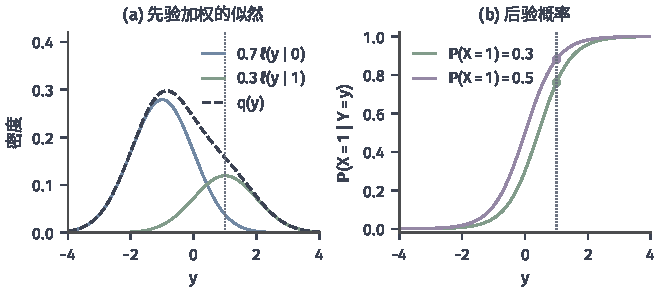
\includegraphics[width=112mm]{figures/02-abstract-mathematics/02-probability-spaces/matplotlib/cond-bayes-posterior/figure.pdf}
  \caption{离散类别与连续观测的Bayes后验。类别$X\in\{0,1\}$，给定$X=0,1$时$Y$分别服从$N(-1,1)$与$N(1,1)$，$\ell$为相应密度。(a)先验$\mathbb P(X=1)=0.3$时的加权似然及其和$q(y)$（虚线）；(b)先验为$0.3$与$0.5$时的后验概率$\mathbb P(X=1\mid Y=y)$，点线标出$y=1$，对应后验约为$0.760$与$0.881$。}
  \label{fig:cond-bayes-posterior}
\end{figure}

\section{条件独立}
\label{sec:cond-independence}

条件分布让我们能够提出一个更细的问题：在已知某些信息之后，另一项观测是否还会改变我们对$X$的判断？
本节用条件概率的乘积分解定义条件独立，给出它的函数判据与核判据，再说明它怎样简化信息依赖，以及它为什么不同于无条件的独立。

\subsection{条件独立的定义与判据}

\paragraph{条件独立的定义}
第~\ref{chap:probability-models}章用联合概率等于边缘概率之积定义独立（定义~\ref{def:pmod-independence}）。
把其中的概率换成给定信息下的条件概率，就得到条件独立。

\begin{definition}[条件独立]
\label{def:cond-independence}
设$X,Y$分别取值于$(E_1,\mathcal E_1)$与$(E_2,\mathcal E_2)$，$\mathcal G\subseteq\mathcal F$是子$\sigma$代数。
若对每个$A\in\mathcal E_1$、$B\in\mathcal E_2$，
\[
  \mathbb P(X\in A,\,Y\in B\mid\mathcal G)=\mathbb P(X\in A\mid\mathcal G)\,\mathbb P(Y\in B\mid\mathcal G)\qquad\text{几乎必然},
\]
则称$X$与$Y$给定$\mathcal G$\term{条件独立}（conditionally independent），记作$X\perp Y\mid\mathcal G$。$\mathcal G=\sigma(Z)$时记作$X\perp Y\mid Z$。
\end{definition}

等式对每一对$(A,B)$各自几乎必然成立，例外零集可以随$(A,B)$变化。
取$\mathcal G=\{\varnothing,\Omega\}$，条件概率就是普通概率，定义回到$X\perp Y$。

\paragraph{有界测试函数判据}
与独立性一样，事件上的乘积分解可以推广到函数。

\begin{lemma}[条件独立的函数判据]
\label{lem:cond-independence-functions}
$X\perp Y\mid\mathcal G$成立，当且仅当对所有有界可测函数$f:E_1\to\mathbb R$、$g:E_2\to\mathbb R$，
\[
  \mathbb E[f(X)g(Y)\mid\mathcal G]=\mathbb E[f(X)\mid\mathcal G]\,\mathbb E[g(Y)\mid\mathcal G]\qquad\text{几乎必然}.
\]
\end{lemma}

\begin{proof}
若函数形式的等式成立，取$f=\mathbb I_A$，$g=\mathbb I_B$即得条件独立。
反过来，若条件独立成立，两边关于$f$和$g$分别线性，所以等式对简单函数$f,g$成立。
对有界可测的$f,g$，取简单函数$f_n\to f$、$g_n\to g$逐点收敛且$|f_n|\leq\sup|f|$、$|g_n|\leq\sup|g|$；由条件控制收敛定理~\ref{thm:cond-dominated}，左边与右边两个因子都几乎必然收敛到相应的极限，于是等式对$f,g$成立。
\end{proof}

\paragraph{用条件核表述}
定义中每一对事件各带一个零集，读起来不如“在每个给定的条件下，联合分布是乘积”直观。
在标准Borel值域下，条件核让后一种说法变得准确。

设$X,Y$取值于标准Borel空间，$Z$取值于可测空间$(D,\mathcal D)$。$E_1\times E_2$仍是标准Borel空间，由定理~\ref{thm:cond-regular-existence}，$(X,Y)$给定$Z$的条件核$K_{XY}$存在。令$K_X(z,A)=K_{XY}(z,A\times E_2)$，$K_Y(z,B)=K_{XY}(z,E_1\times B)$，它们分别是$X$与$Y$给定$Z$的条件核。

\begin{theorem}[条件独立的核判据]
\label{thm:cond-independence-kernel}
在上述设定下，$X\perp Y\mid Z$成立，当且仅当存在$P_Z$零集$N$，使对每个$z\notin N$，
\[
  K_{XY}(z,\cdot)=K_X(z,\cdot)\otimes K_Y(z,\cdot).
\]
\end{theorem}

\begin{proof}
若核等式成立，在矩形$A\times B$上取值并代入$z=Z$，得$\mathbb P(X\in A,Y\in B\mid Z)=K_X(Z,A)K_Y(Z,B)=\mathbb P(X\in A\mid Z)\mathbb P(Y\in B\mid Z)$几乎必然成立。
反过来，取$E_1,E_2$各自的可数生成$\pi$系统$\mathcal C_1,\mathcal C_2$（分别包含$E_1,E_2$）。矩形族$\{A\times B:A\in\mathcal C_1,B\in\mathcal C_2\}$是可数$\pi$系统，并生成乘积$\sigma$代数。对其中每个矩形，条件独立给出$K_{XY}(z,A\times B)=K_X(z,A)K_Y(z,B)$在一个$P_Z$零集外成立；可数个零集的并$N$仍是零集。对$z\notin N$，两个概率测度$K_{XY}(z,\cdot)$与$K_X(z,\cdot)\otimes K_Y(z,\cdot)$在生成$\pi$系统上一致，由定理~\ref{thm:measure-uniqueness}，它们相等。
\end{proof}

定理说：固定一个有效的条件输入$z$之后，联合分布中不再有超出两个边缘分布的依赖。
证明中的关键仍然是可数生成族：只有可数个矩形的例外零集可以合并。
所以不要把每个事件对各自成立的版本等式，直接当作已经逐点一致的核等式；从前者到后者，需要先有条件核，再借助可数生成族。

\subsection{条件独立与信息简化}

\paragraph{已知$Z$后$Y$不再提供信息}
条件独立最常用的推论是删去多余的条件。
直观上，若给定$Z$后$X$与$Y$独立，那么已经知道$Z$时，再知道$Y$不会改变对$X$的平均判断。

\begin{theorem}[条件独立下的信息简化]
\label{thm:cond-independence-reduction}
设$X,Y,Z$是随机对象。若$X\perp Y\mid Z$，则对每个有界可测函数$f$，
\[
  \mathbb E[f(X)\mid Y,Z]=\mathbb E[f(X)\mid Z]\qquad\text{几乎必然}.
\]
反之，若上式对所有有界可测$f$成立，则$X\perp Y\mid Z$。
\end{theorem}

\begin{proof}
记$W=\mathbb E[f(X)\mid Z]$，它对$\sigma(Z)\subseteq\sigma(Y,Z)$可测。事件$\{Y\in B\}\cap\{Z\in C\}$构成包含$\Omega$并生成$\sigma(Y,Z)$的$\pi$系统，由引理~\ref{lem:cond-pi-check}，只需在这些事件上检验积分。利用全期望公式、函数判据（引理~\ref{lem:cond-independence-functions}）和提出已知因子，
\[
  \begin{aligned}
  \mathbb E[f(X)\mathbb I_B(Y)\mathbb I_C(Z)]
  &=\mathbb E\bigl[\mathbb I_C(Z)\,\mathbb E[f(X)\mathbb I_B(Y)\mid Z]\bigr]\\
  &=\mathbb E\bigl[\mathbb I_C(Z)\,W\,\mathbb E[\mathbb I_B(Y)\mid Z]\bigr]\\
  &=\mathbb E\bigl[\mathbb E[W\mathbb I_C(Z)\mathbb I_B(Y)\mid Z]\bigr]
  =\mathbb E[W\mathbb I_B(Y)\mathbb I_C(Z)],
  \end{aligned}
\]
其中第三个等号把有界的$\sigma(Z)$可测因子$W\mathbb I_C(Z)$放回条件期望之内。所以$W=\mathbb E[f(X)\mid Y,Z]$。

反过来，设上式对所有有界可测$f$成立。对有界可测$g$，由塔式法则（$\sigma(Z)\subseteq\sigma(Y,Z)$）与提出已知因子，
\[
  \begin{aligned}
  \mathbb E[f(X)g(Y)\mid Z]&=\mathbb E\bigl[g(Y)\,\mathbb E[f(X)\mid Y,Z]\bigm|Z\bigr]\\
  &=\mathbb E\bigl[g(Y)\,\mathbb E[f(X)\mid Z]\bigm|Z\bigr]=\mathbb E[f(X)\mid Z]\,\mathbb E[g(Y)\mid Z],
  \end{aligned}
\]
由引理~\ref{lem:cond-independence-functions}得$X\perp Y\mid Z$。
\end{proof}

反向判别需要对\emph{全部}有界可测$f$成立；只对某一个$f$成立，例如只知道条件均值不依赖$Y$，并不能推出条件独立。

\begin{example}[共享类别的两个比特]
\label{ex:cond-shared-class}
设类别$Z\in\{0,1\}$，$\mathbb P(Z=0)=\mathbb P(Z=1)=\frac12$。给定$Z=z$时，$X,Y$独立且都服从$\operatorname{Bernoulli}(p_z)$，取$p_0=0.2$，$p_1=0.8$。
按构造$X\perp Y\mid Z$，由定理~\ref{thm:cond-independence-reduction}，
\[
  \mathbb P(X=1\mid Y,Z)=\mathbb P(X=1\mid Z)=p_Z.
\]
知道类别后，$Y$的取值不再改变$X=1$的概率。
可是不给定$Z$时，$\mathbb P(X=1)=\mathbb P(Y=1)=0.5$，而
\[
  \mathbb P(X=1,Y=1)=\tfrac12(0.2^2+0.8^2)=0.34\neq0.25,
\]
所以$X$与$Y$并不独立：$\mathbb P(X=1\mid Y=1)=0.68$。$Y=1$让类别$1$更可信，从而间接提高了$X=1$的概率。
\end{example}

\paragraph{条件化可能产生依赖}
条件独立与独立互不蕴含。上例是条件独立而不独立；反方向的例子来自第~\ref{chap:probability-models}章的两个独立公平比特（示例~\ref{ex:pmod-xor-bits}）。
设$X,Y$独立且各以概率$\frac12$取$0,1$，$Z=X\oplus Y$为模二和。那里用这个例子区分两两独立与相互独立；这里用它检验条件化的影响。
给定$Z=0$，必有$Y=X$，于是
\[
  \begin{aligned}
  \mathbb P(X=1,Y=1\mid Z=0)&=\tfrac12,\\
  \mathbb P(X=1\mid Z=0)\,\mathbb P(Y=1\mid Z=0)&=\tfrac12\times\tfrac12=\tfrac14.
  \end{aligned}
\]
这里$\mathbb P(X=1\mid Z=0)=\frac12$，因为$X$与$Z$独立。给定$Z$后知道$X$就确定了$Y$，原本的独立性消失了。

图~\ref{fig:cond-independence-tables}并排列出两个例子的联合概率表。
上排中，给定$Z=0$或$Z=1$时的表都是外积，但按$Z$平均后对角格变大，不再是边缘的乘积；下排中，无条件的表是均匀的乘积，给定$Z$后质量集中到对角或反对角，不再是乘积。

\begin{figure*}[htbp]
  \centering
  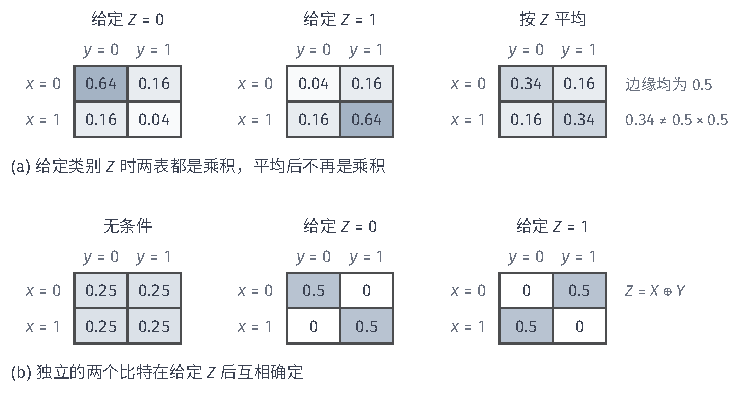
\includegraphics[width=125mm]{figures/02-abstract-mathematics/02-probability-spaces/tikz/cond-independence-tables/figure.pdf}
  \caption{条件独立与条件化后出现的依赖，表中为$(X,Y)$的联合概率，底色深浅与概率成正比。(a)$\mathbb P(Z=0)=\mathbb P(Z=1)=\frac12$，给定$Z=z$时$X,Y$独立同分布于$\operatorname{Bernoulli}(p_z)$，$p_0=0.2$，$p_1=0.8$：两张条件表都是乘积，平均后$\mathbb P(X=1,Y=1)=0.34$，大于边缘乘积$0.25$。(b)$X,Y$为独立公平比特，$Z=X\oplus Y$：无条件表为乘积，给定$Z=0$或$Z=1$后只剩两格。}
  \label{fig:cond-independence-tables}
\end{figure*}

条件独立始终是给定联合分布之内的关系，它说明的是“已知$Z$时$Y$对$X$不再提供信息”。
它本身不说明改变$Y$是否会影响$X$：干预、因果效应及其识别需要额外的模型与假设，归卷四推断与因果识别部分讨论。

\section{本章小结}
\label{sec:cond-summary}

章首问的是：观测取连续值、每个观测值的概率都是零时，给定观测的平均和分布指什么。
本章的回答从有限分组中的条件平均开始。
分组平均有两项性质：只依赖可用的信息，在每个可观察事件上保持积分总量。
条件期望把这两项性质原样作为定义，完全不做除法，因此对零概率的观测值同样有意义；Radon--Nikodym定理保证它对任意子$\sigma$代数存在，并且几乎必然唯一。
给定观测$Y$时，Doob--Dynkin引理把它写成观测值的函数$h(Y)$，$h$在$P_Y$几乎处处的意义下确定。

从同一个定义出发，我们得到可以直接使用的几组规则。
线性、保序、提出已知因子和塔式法则支撑日常计算，其中提出因子需要$X$与$HX$可积，塔式法则需要两个信息有包含关系。
条件Jensen不等式给出矩与平均误差的收缩；条件均方误差分解说明，在只依据给定信息的平方可积预测中，条件平均的均方误差最小。
条件单调收敛、条件Fatou与条件控制收敛在固定信息下交换条件期望与极限，控制变量可积是避免$\infty-\infty$的条件。

第二个问题是怎样用一个对象同时给出所有事件的条件概率。
概率核提供了这样的对象：它由输入分布构造联合分布，复合时对中间状态求平均。
条件分布就是满足逐事件条件的概率核；逐事件的条件概率总是存在，但把它们拼成分布需要检查取值空间的可测结构，本书使用的充分条件是取值于标准Borel空间。
条件核在一个共同的$P_Y$零集外唯一，用它可以统一计算各种条件平均，有密度时由条件密度或Bayes公式写出。
条件独立则用条件核表达“已知$Z$后$Y$不再提供信息”，它与独立互不蕴含，也不等同于因果关系。

零概率观测值上的版本自由贯穿全章：条件期望、条件核和条件密度都只在几乎处处意义下确定。
第~\ref{chap:random-variable-convergence}章将用本章的收缩估计和条件极限定理研究随机变量列的平均收敛；条件期望的投影结构留给第~\ref{part:function-spaces}部分，随时间增加的信息与过程模型留给卷三。
